\section{Three-dimensional bump-in-channel}
\label{sec:syn3dbump}
The third verification case from the TMR website that was investigated was the three-dimensional bump-in-channel, which is available on~\cite{tmr} under the name ``3D Bump-in-channel''. This case was only simulated with syn3D.

The problem domain and flow conditions are shown in~\Cref{fig:3dbump}. While the website provides five sets of grids for this case as well, only results from the finest three grids are shown.
\begin{figure}
    \centering
    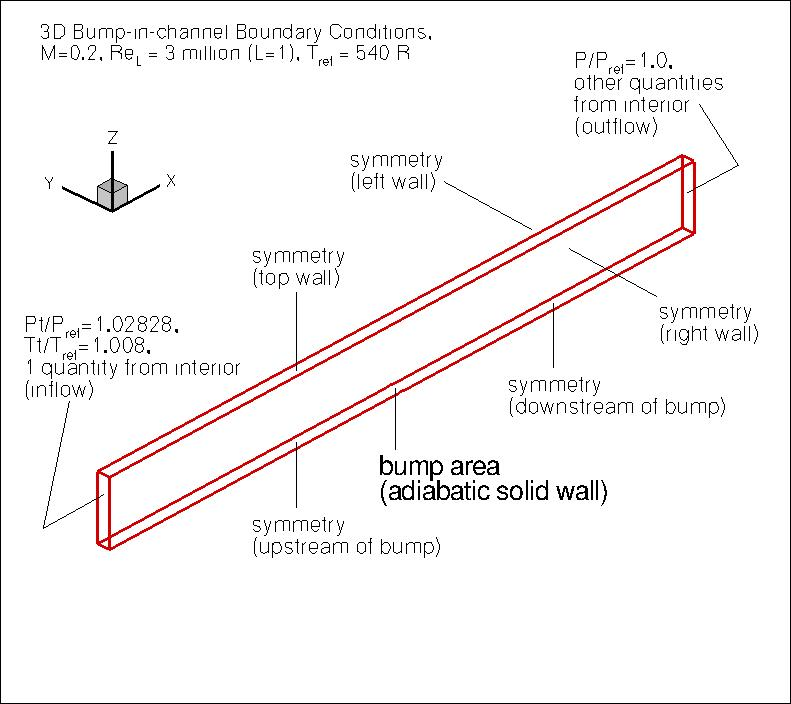
\includegraphics[width=0.7\textwidth]{figs/3dbump/bump3dBCpic1.jpg}
    \caption{Turbulent three-dimensional bump case~\cite{tmr}.}
    \label{fig:3dbump}
\end{figure}

The number of elements of the finest available grid exceeds 1.5 million and the residual could not be converged past $10^{-2}$ after over 6 days of computation with 64 cores, which is typically insufficient for the purposes of validation -- results are shown nonetheless.

\Cref{tab:syn3dbump} compares force coefficients and shows relatively good agreement. \Cref{fig:syn3dbumpcnv} shows the convergence for the finest three grids.
\begin{table}[ht!]
\centering
\caption{3D Bump (syn3D): Comparison of force coefficients for the three-dimensional bump.}
\label{tab:syn3dbump}
\begin{tabular}{@{}l cccc@{}}
\toprule
Solver & $C_L$ & $C_D$ & $C_{Dv}$ & $C_{Dp}$ \\  \midrule
CFL3D & 0.0250 & 0.0036  & 0.0032 & 0.0004  \\
syn3D &  0.0258 & 0.0035  & 0.0031 & 0.0004  \\
\bottomrule
\end{tabular}
\end{table}
 \begin{figure}[ht!]
\centering
\begin{subfigure}{.45\textwidth}
  \centering
  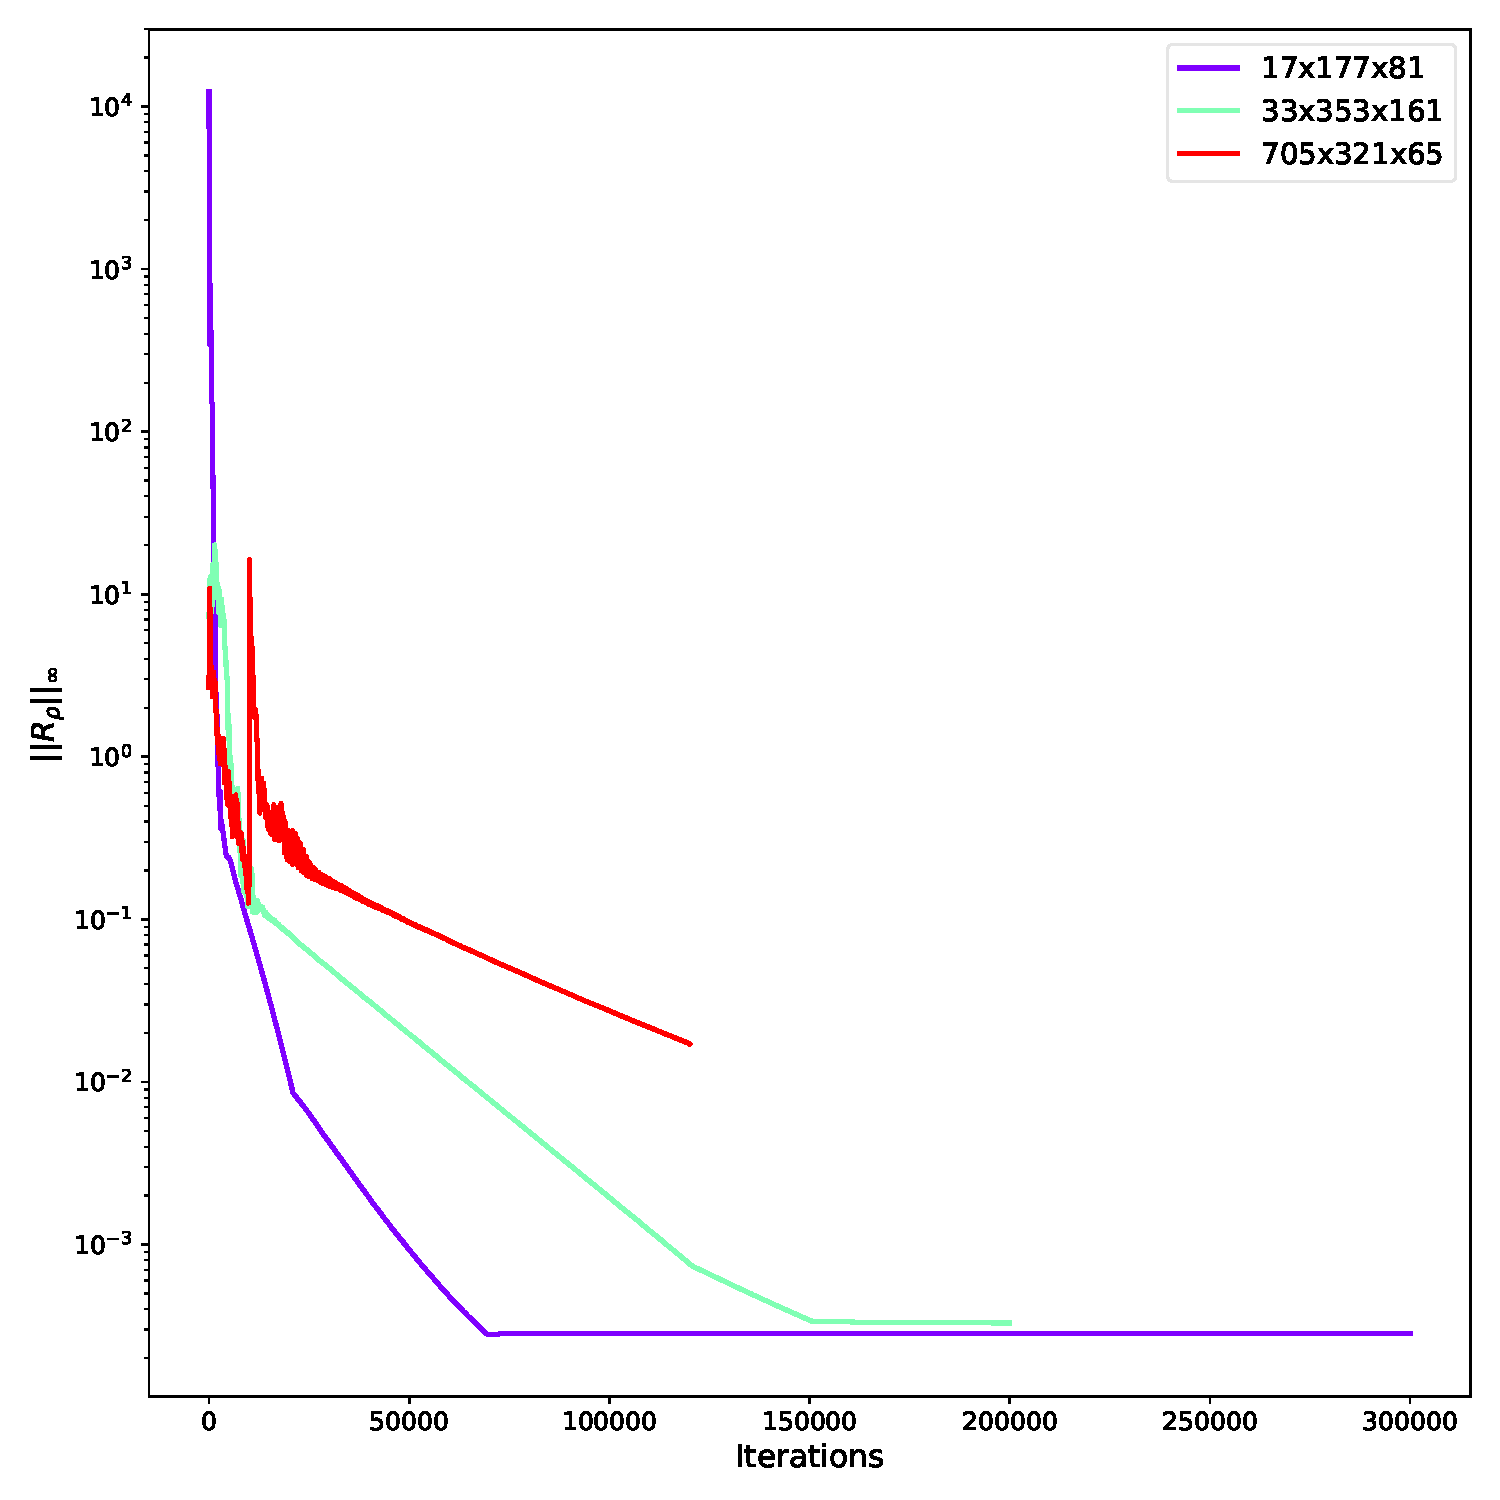
\includegraphics[width=1.0\textwidth]{figs/3dbump/convergenceRho.pdf}
  \caption{Maximum density residual.}
\end{subfigure}%
\begin{subfigure}{.45\textwidth}
  \centering
  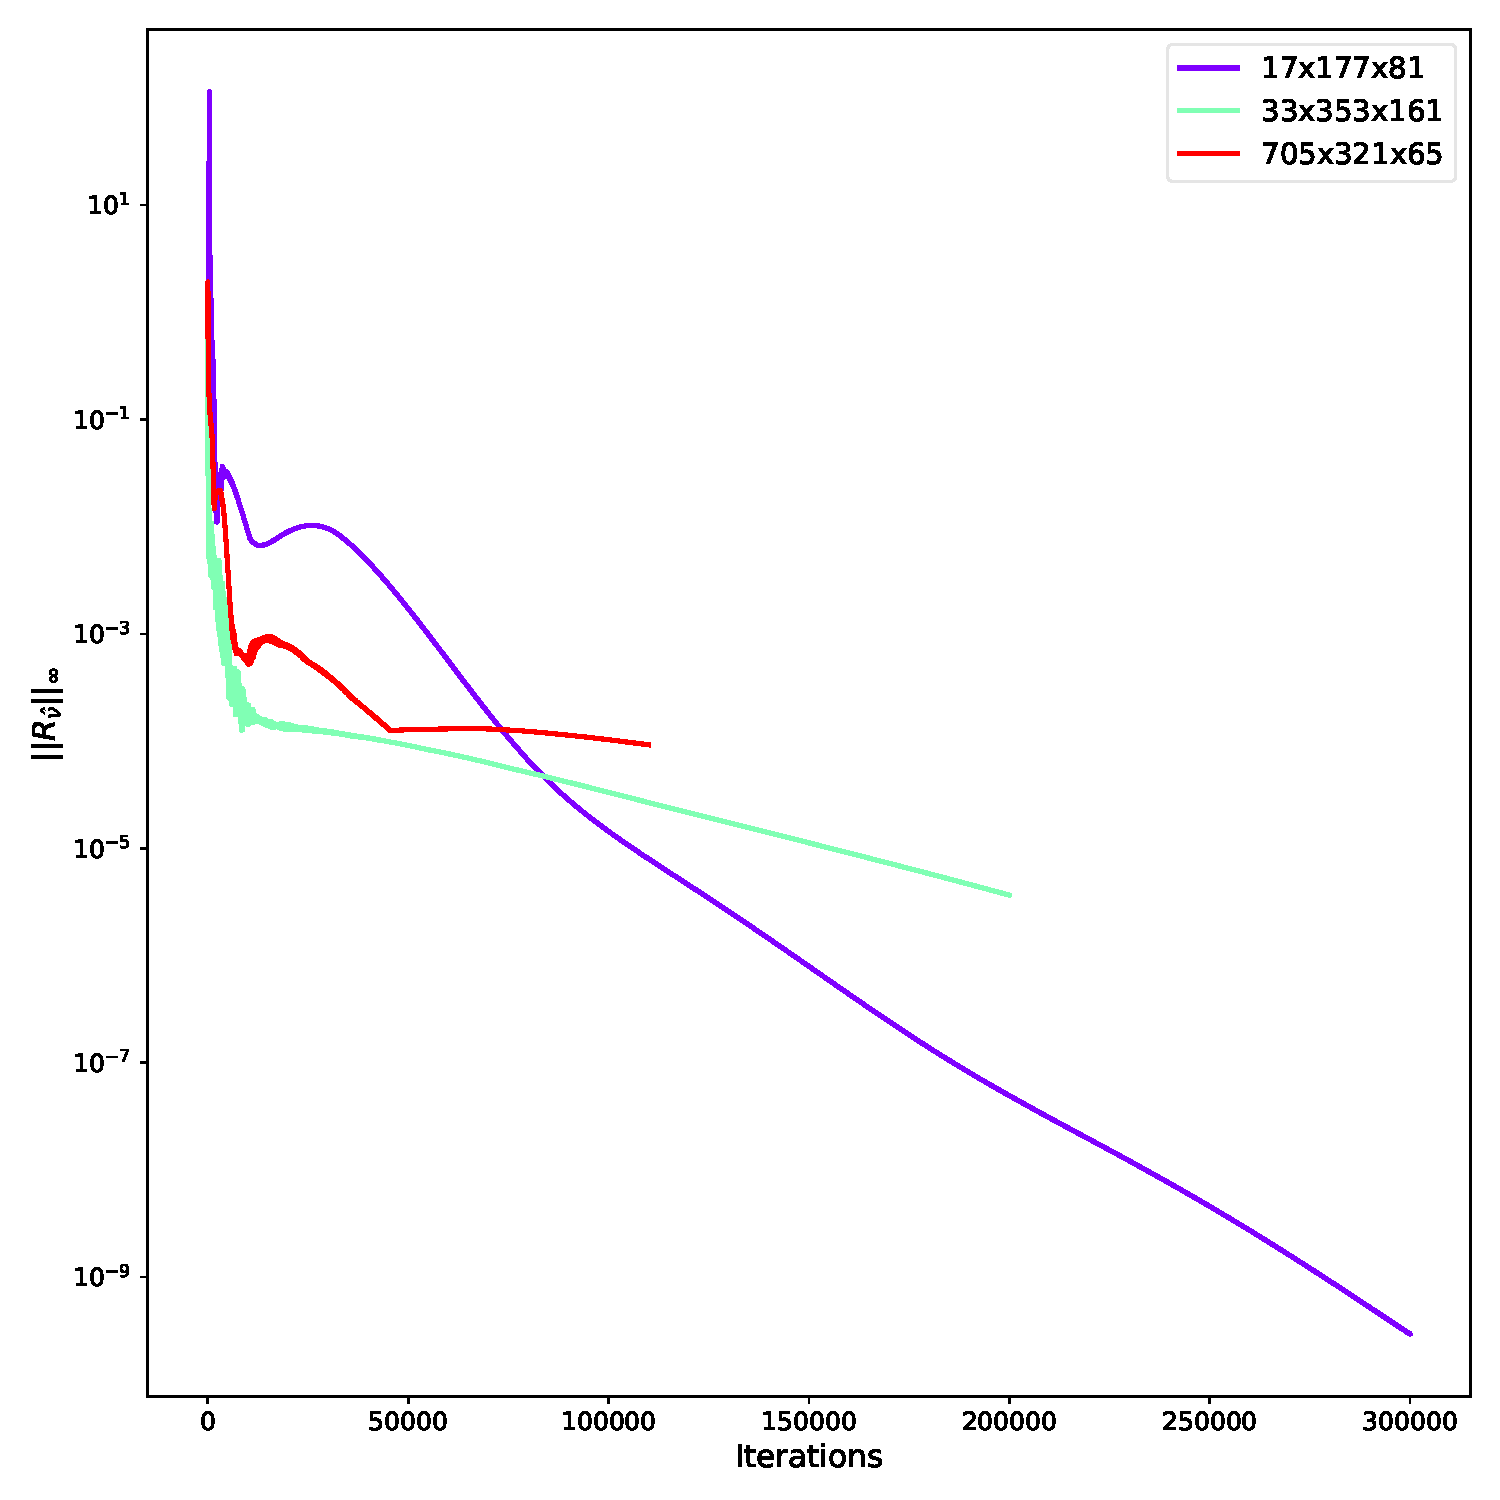
\includegraphics[width=1.0\textwidth]{figs/3dbump/convergencesa.pdf}
  \caption{Maximum turbulent variable residual.}
\end{subfigure}
\caption{3D Bump (syn3D): Convergence of flow and turbulence variables.}
\label{fig:syn3dbumpcnv}
\end{figure}

 \begin{figure}[ht!]
\centering
\begin{subfigure}{.45\textwidth}
  \centering
  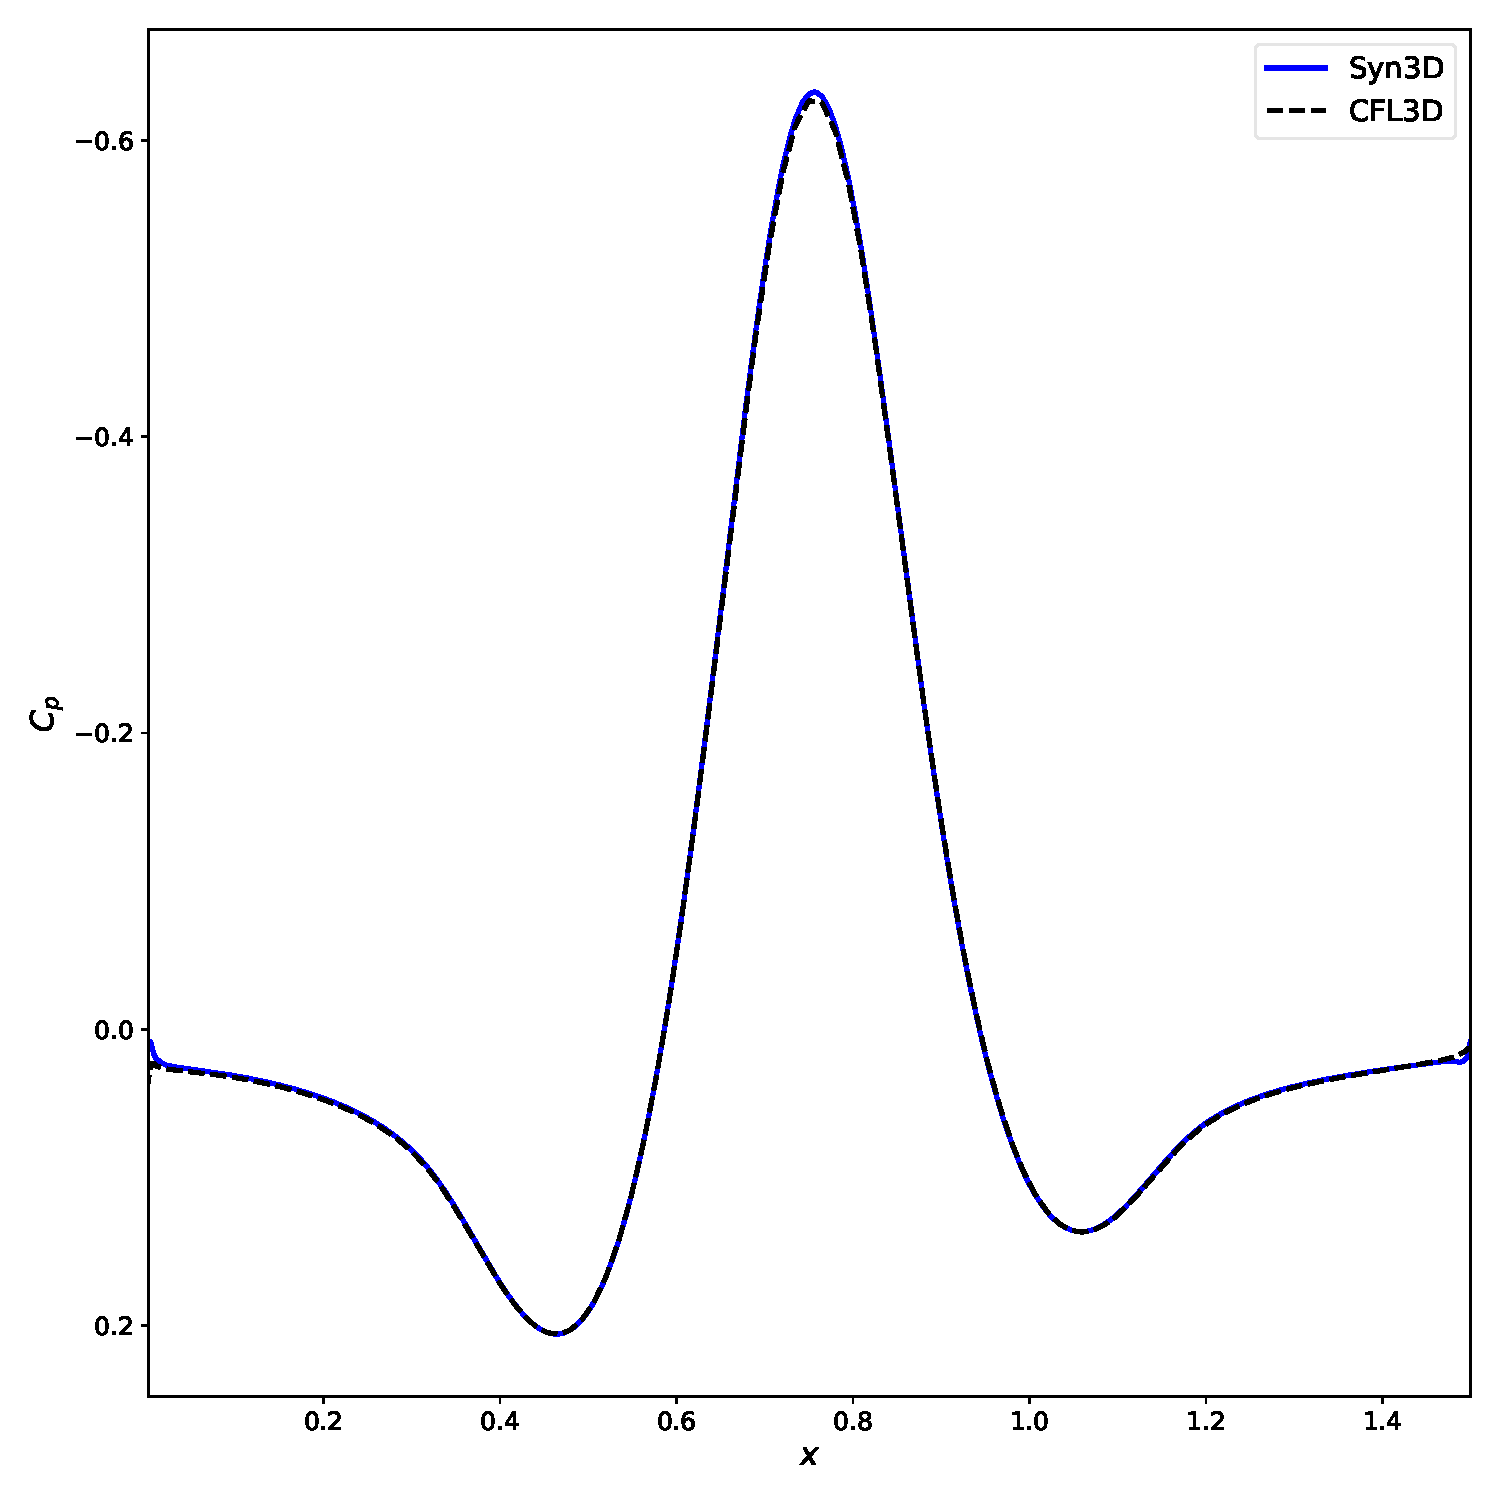
\includegraphics[width=1.0\textwidth]{figs/3dbump/cop001.pdf}
  \caption{$y=0.01$}
\end{subfigure}%
\begin{subfigure}{.45\textwidth}
  \centering
  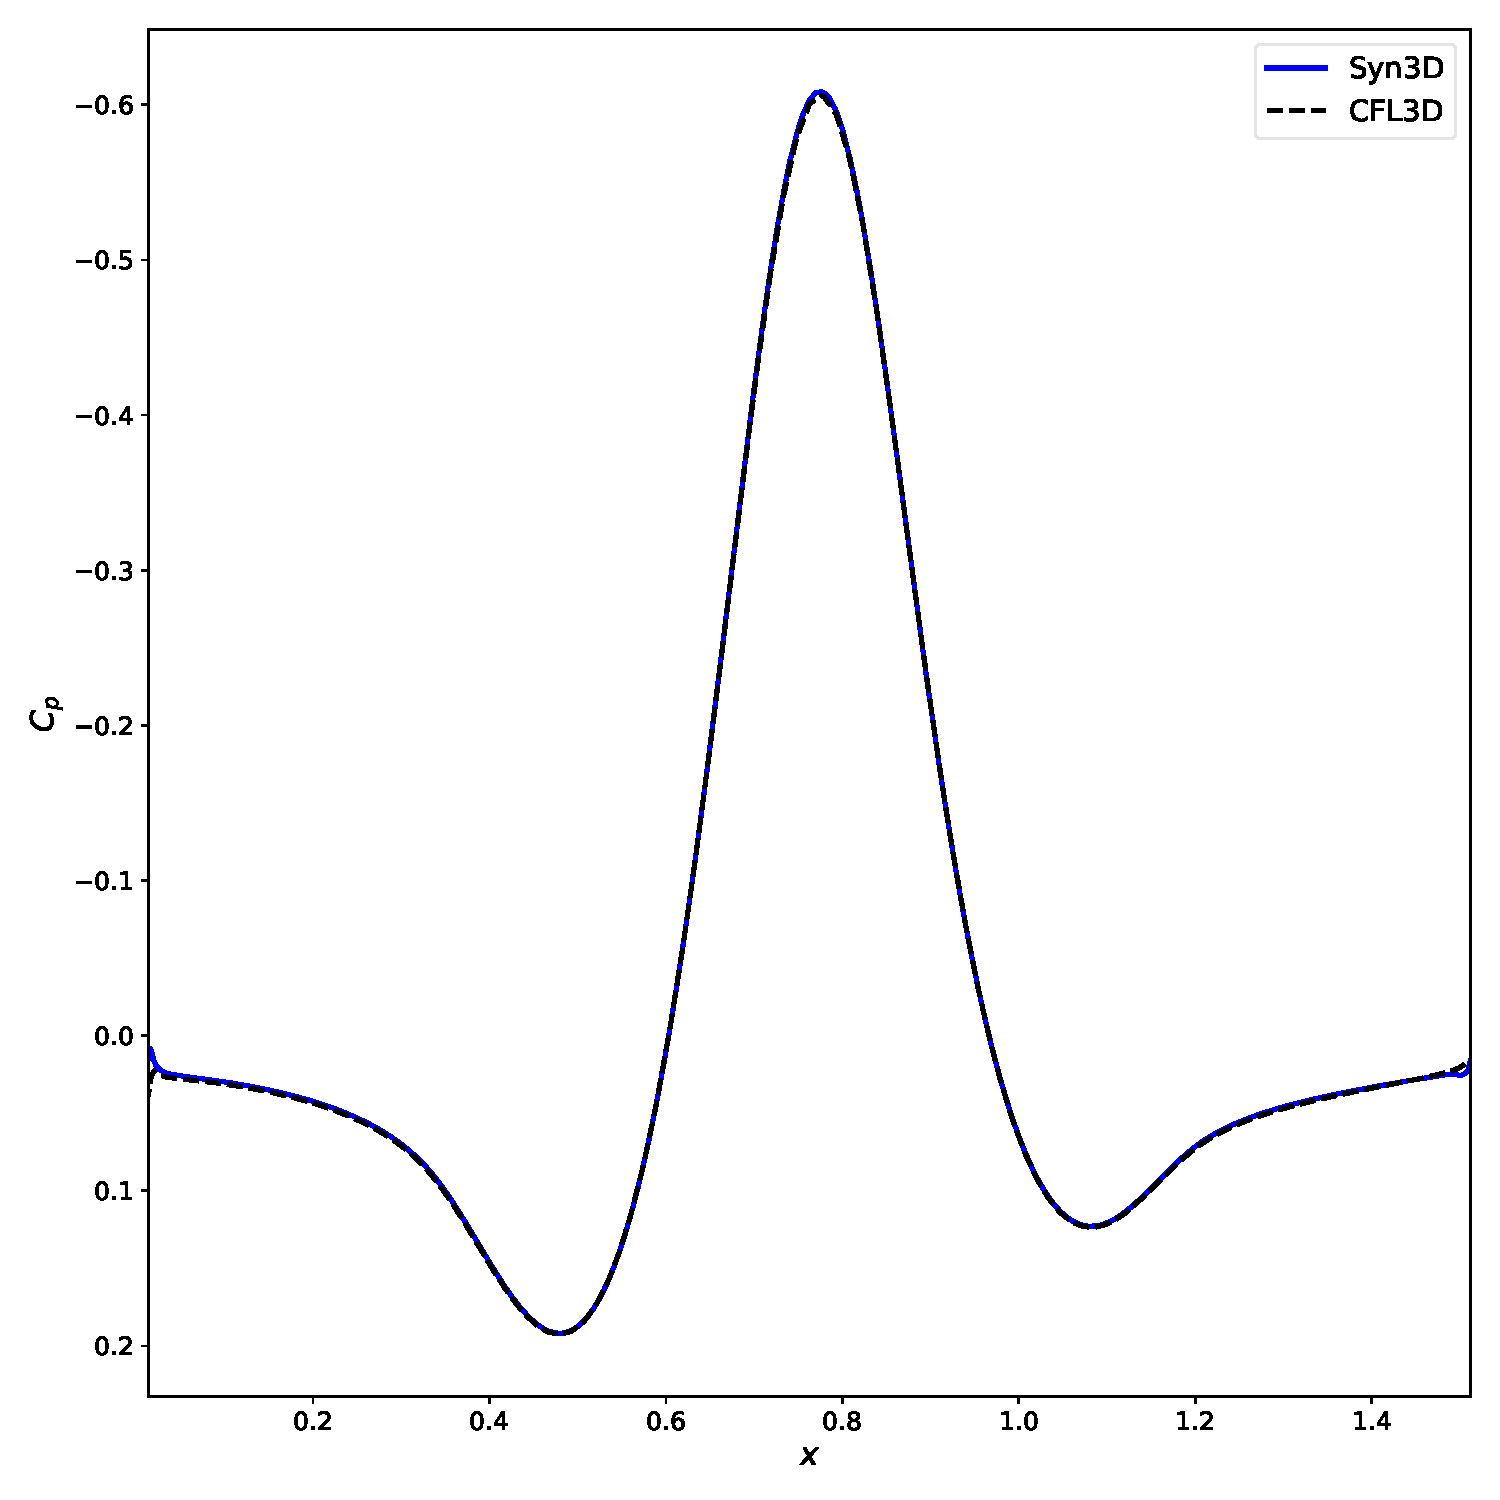
\includegraphics[width=1.0\textwidth]{figs/3dbump/cop015.pdf}
  \caption{$y=0.15$}
\end{subfigure}
\\
\begin{subfigure}{.45\textwidth}
  \centering
  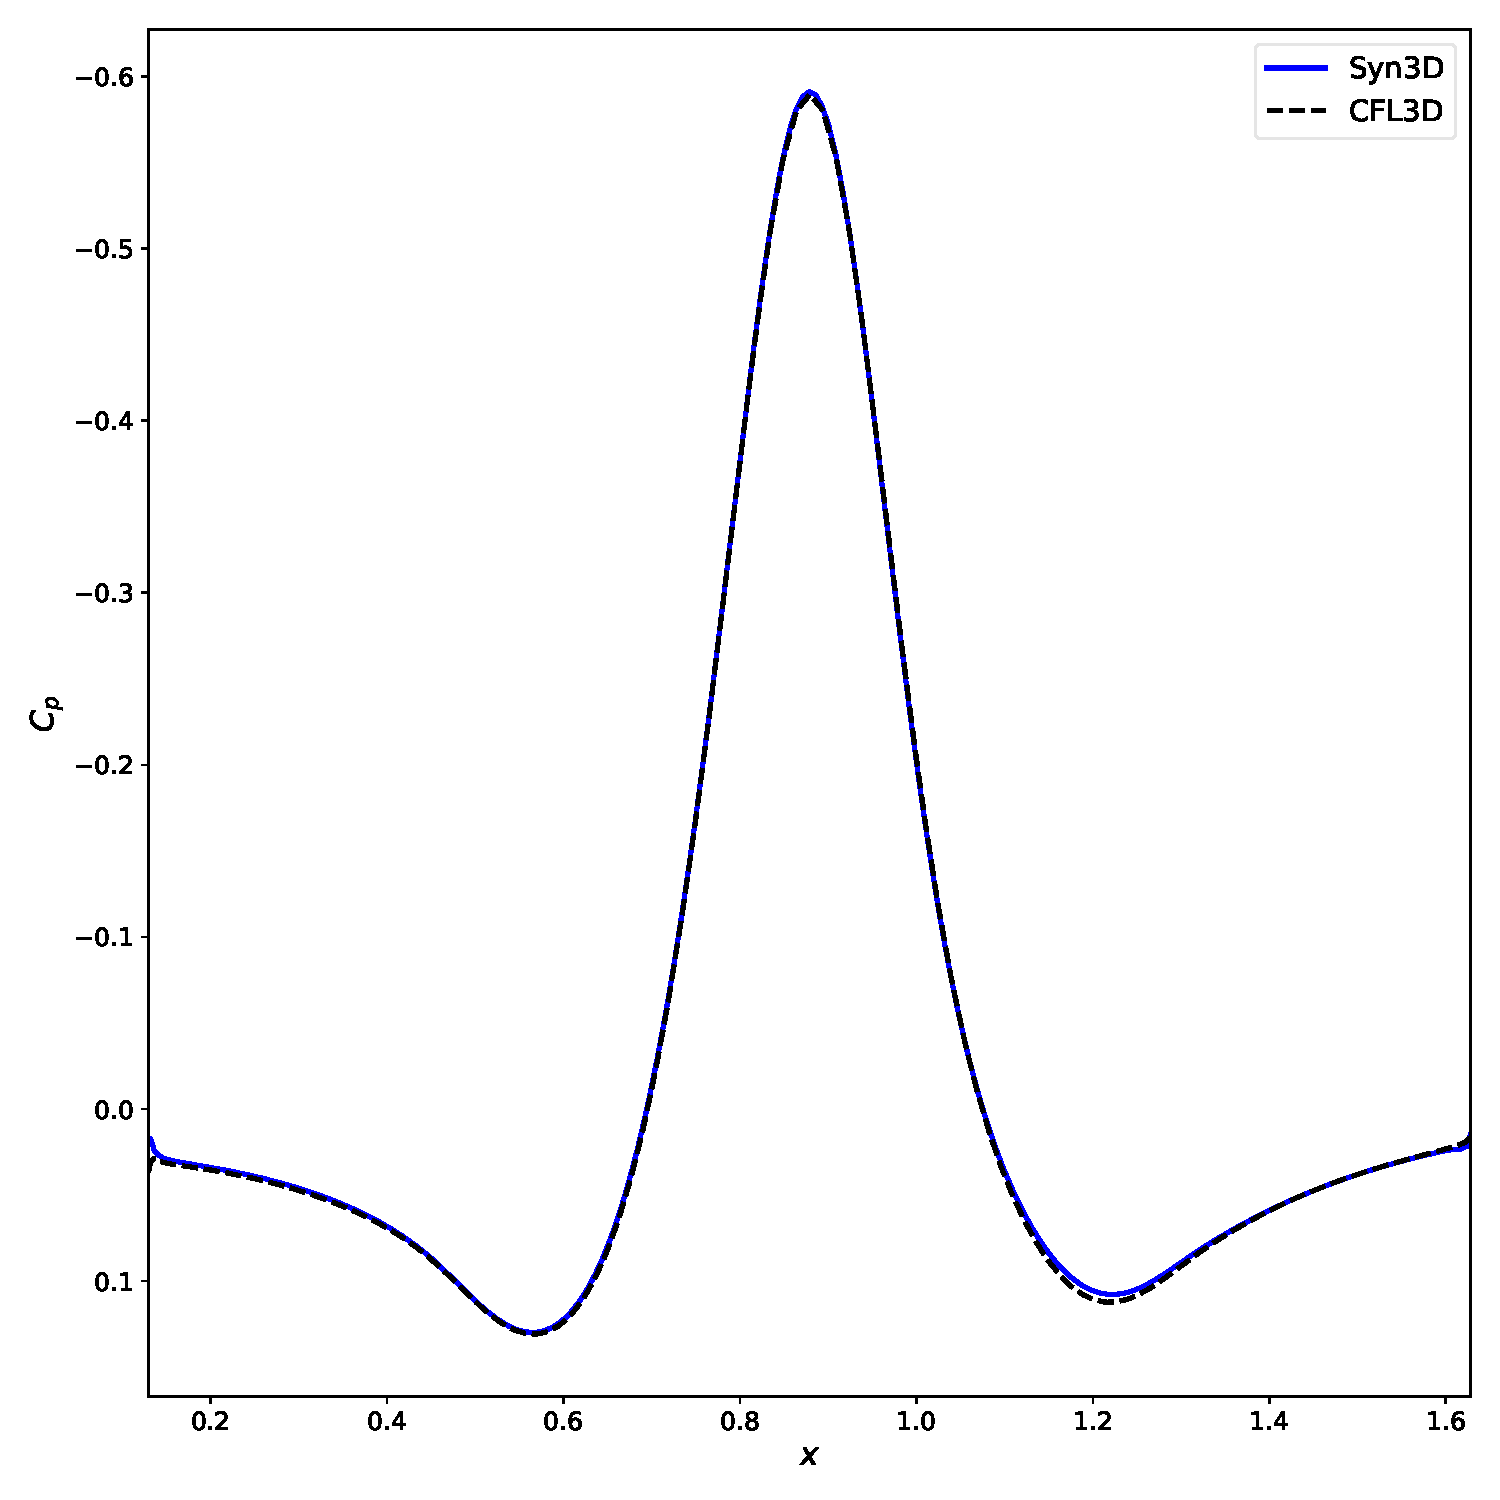
\includegraphics[width=1.0\textwidth]{figs/3dbump/cop030.pdf}
  \caption{$y=0.3$}
\end{subfigure}%
\begin{subfigure}{.45\textwidth}
  \centering
  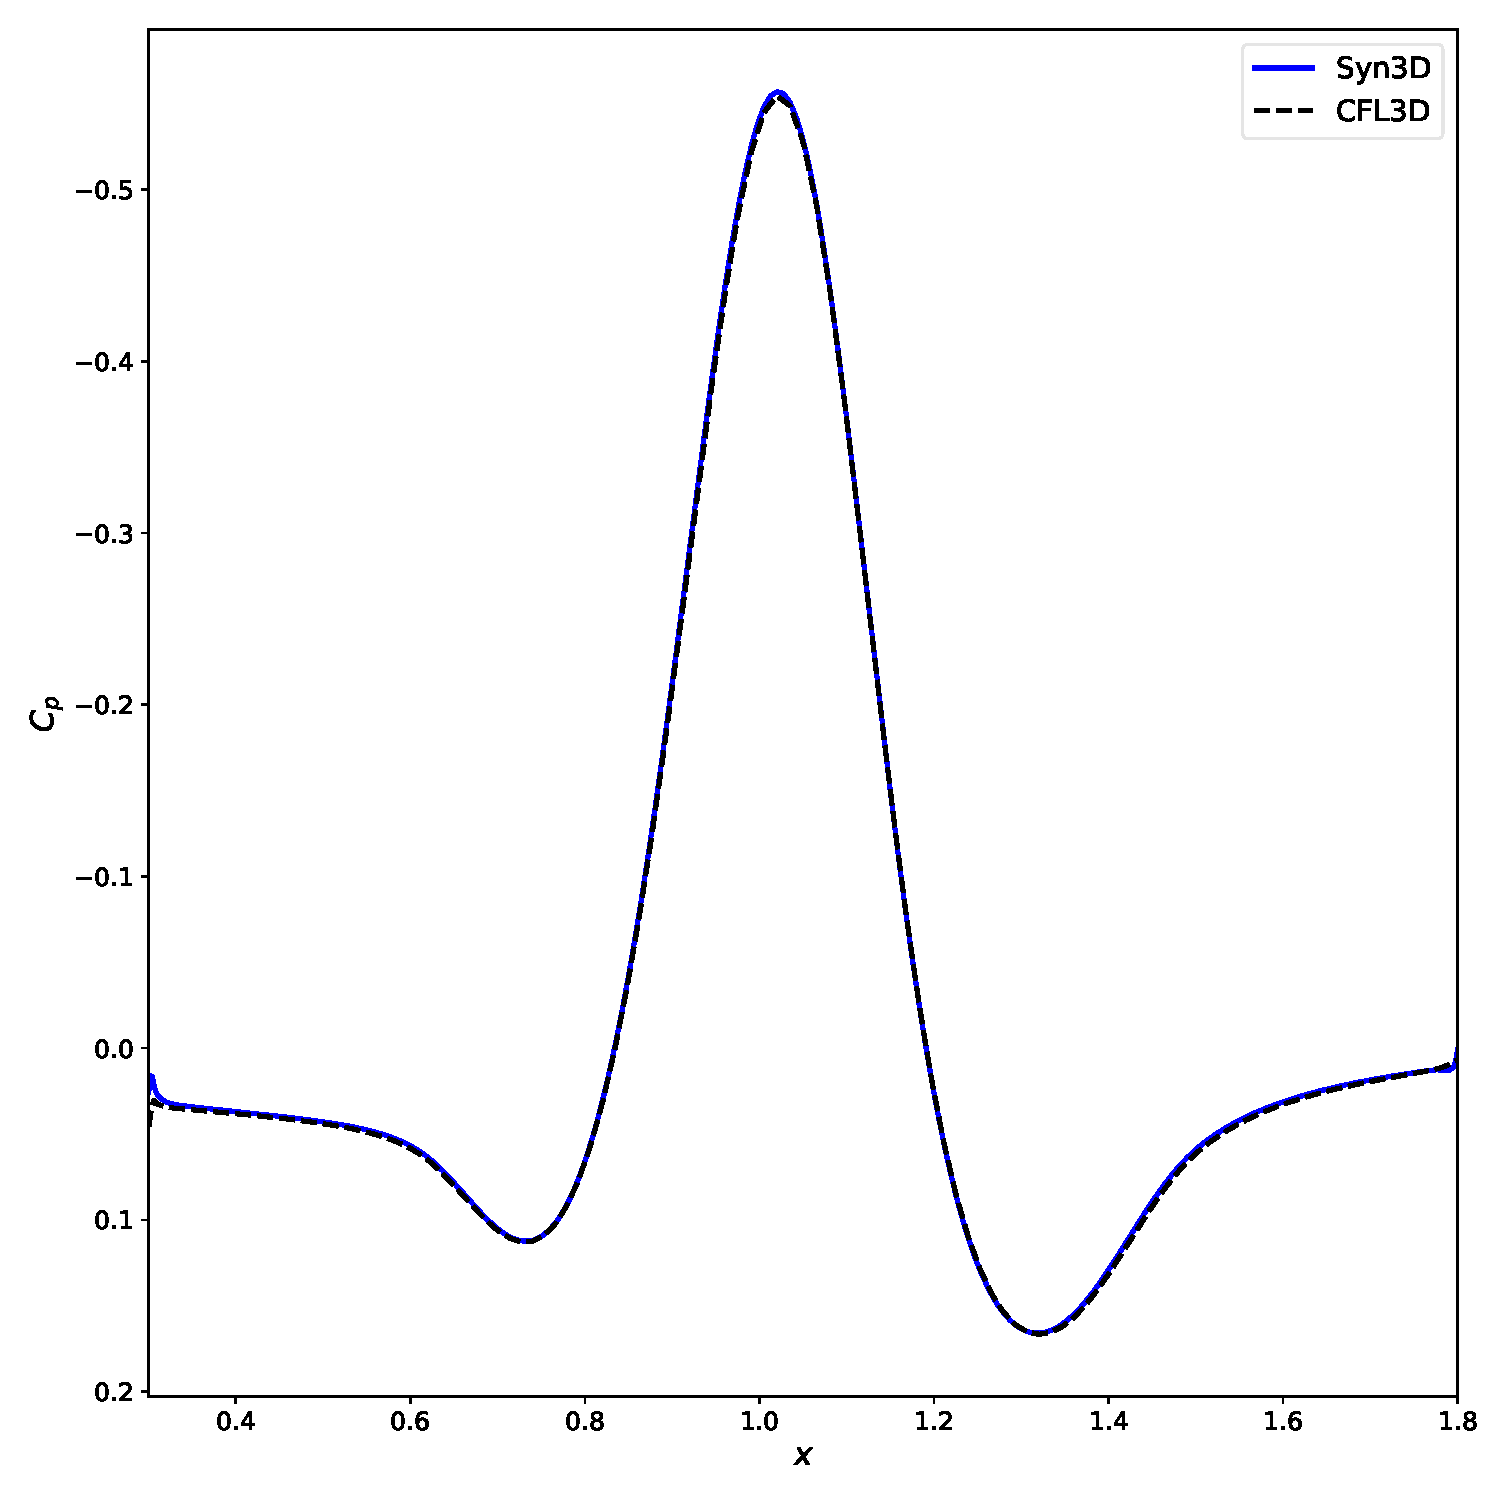
\includegraphics[width=1.0\textwidth]{figs/3dbump/cop050.pdf}
  \caption{$y=0.50$}
\end{subfigure}
\caption{3D Bump (syn3D): Comparison of coefficient of pressure distribution at various cross-sections.}
\label{fig:syn3dbumpcp}
\end{figure}
\Cref{fig:syn3dbumpcp} compares $C_p$ at four fixed values of $y$. \Cref{fig:syn3dbumpmut03,fig:syn3dbumpmut12} show contour plots of the dimensionless eddy viscosity at $x=0.3$ and $x=1.2$ respectively. \Cref{fig:syn3dbumpmut} compares dimensionless eddy viscosity profiles at various locations. The plots are similar in trend to those of the two-dimensional bump, but vary due to the three-dimensional geometry of the bump. While the eddy viscosity is, as in previous cases, over-predicted by syn3D, \Cref{fig:syn3dbumpbad} displays a large discrepancy between syn3D and CFL3D.

\begin{figure}[ht!]
\centering
\begin{subfigure}{.45\textwidth}
  \centering
  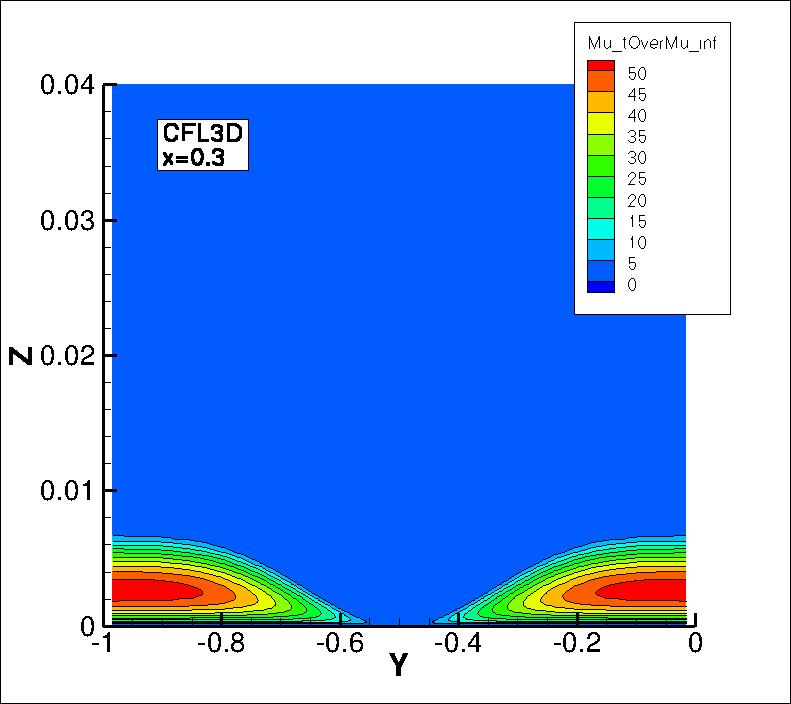
\includegraphics[width=1.0\textwidth]{figs/3dbump/mut_03_cfl3d.jpg}
  \caption{CFL3D}
\end{subfigure}%
\begin{subfigure}{.45\textwidth}
  \centering
  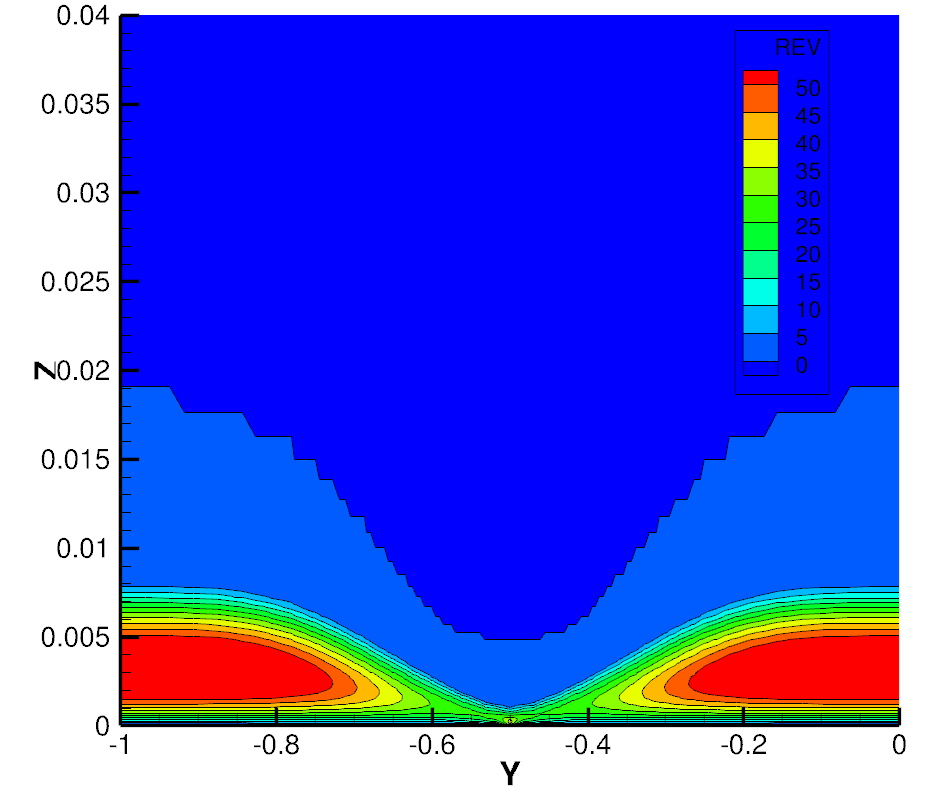
\includegraphics[width=1.0\textwidth]{figs/3dbump/x03Rev.png}
  \caption{syn3D}
\end{subfigure}
\caption{3D Bump (syn3D): Contours of $\frac{\mu_t}{\mu_{\infty}}$ at $x=0.3$}
\label{fig:syn3dbumpmut03}
\end{figure}

\begin{figure}[ht!]
\centering
\begin{subfigure}{.45\textwidth}
  \centering
  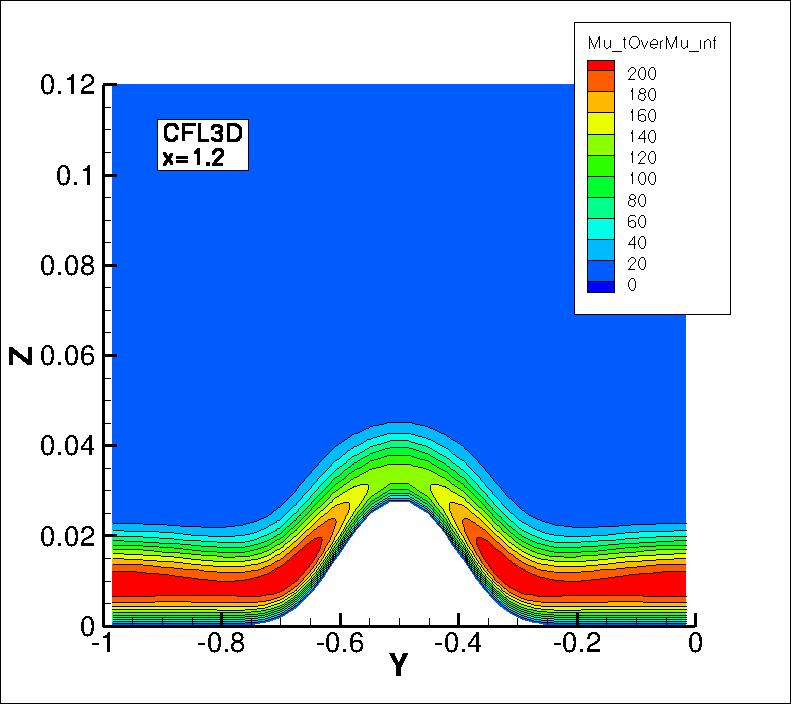
\includegraphics[width=1.0\textwidth]{figs/3dbump/mut_12_cfl3d.jpg}
  \caption{CFL3D}
\end{subfigure}%
\begin{subfigure}{.45\textwidth}
  \centering
  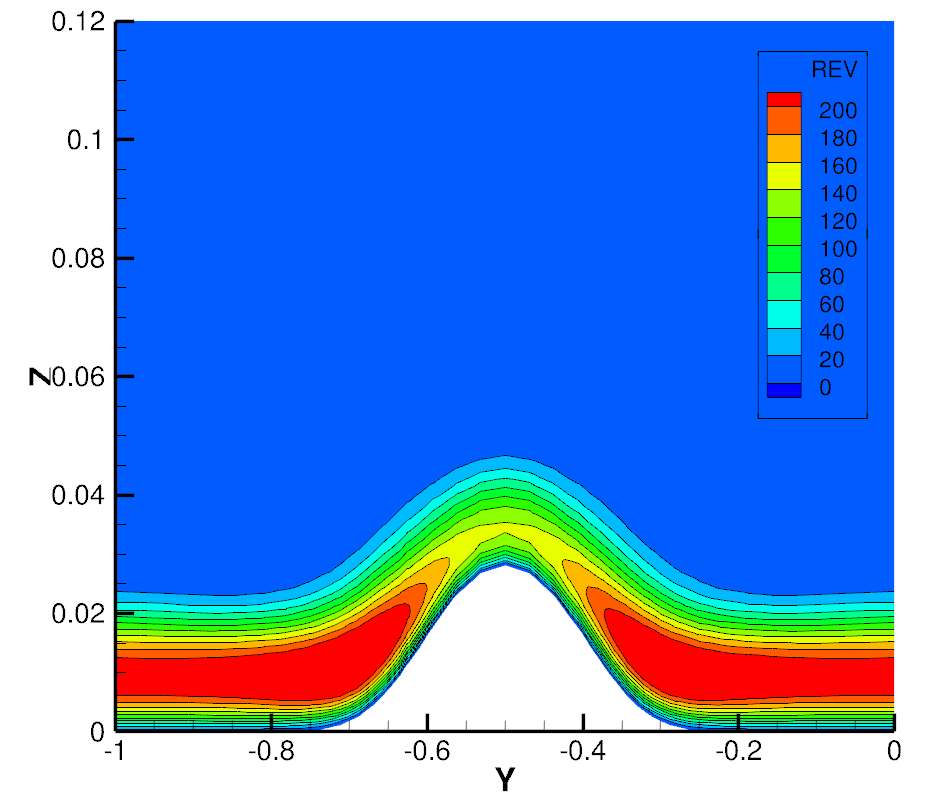
\includegraphics[width=1.0\textwidth]{figs/3dbump/x12Rev.png}
  \caption{syn3D}
\end{subfigure}
\caption{3D Bump (syn3D): Contours of $\frac{\mu_t}{\mu_{\infty}}$ at $x=1.2$}
\label{fig:syn3dbumpmut12}
\end{figure}

\begin{figure}[ht!]
\centering
\begin{subfigure}{.45\textwidth}
  \centering
  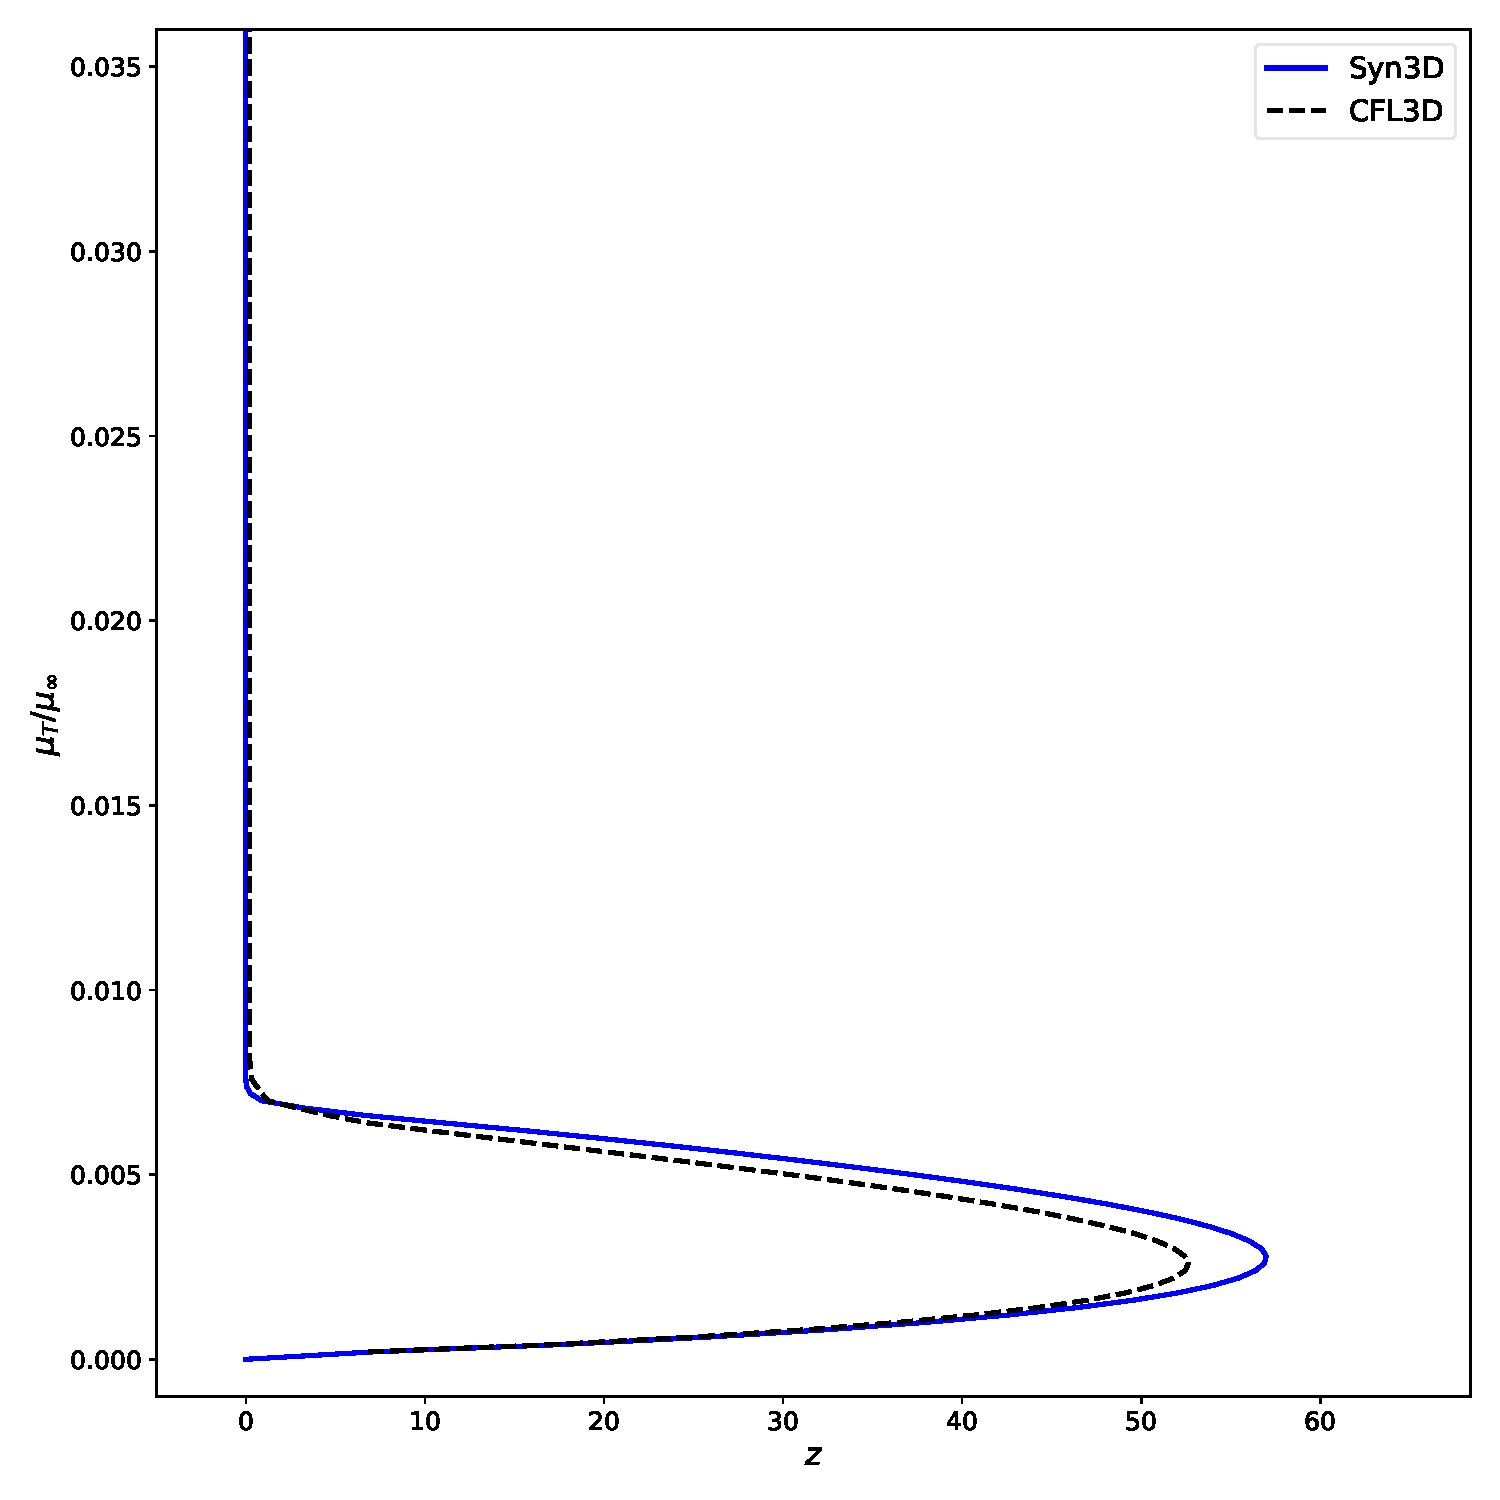
\includegraphics[width=1.0\textwidth]{figs/3dbump/x03y01REV.pdf}
  \caption{$x=0.3, y=-0.1$}
\end{subfigure}%
\begin{subfigure}{.45\textwidth}
  \centering
  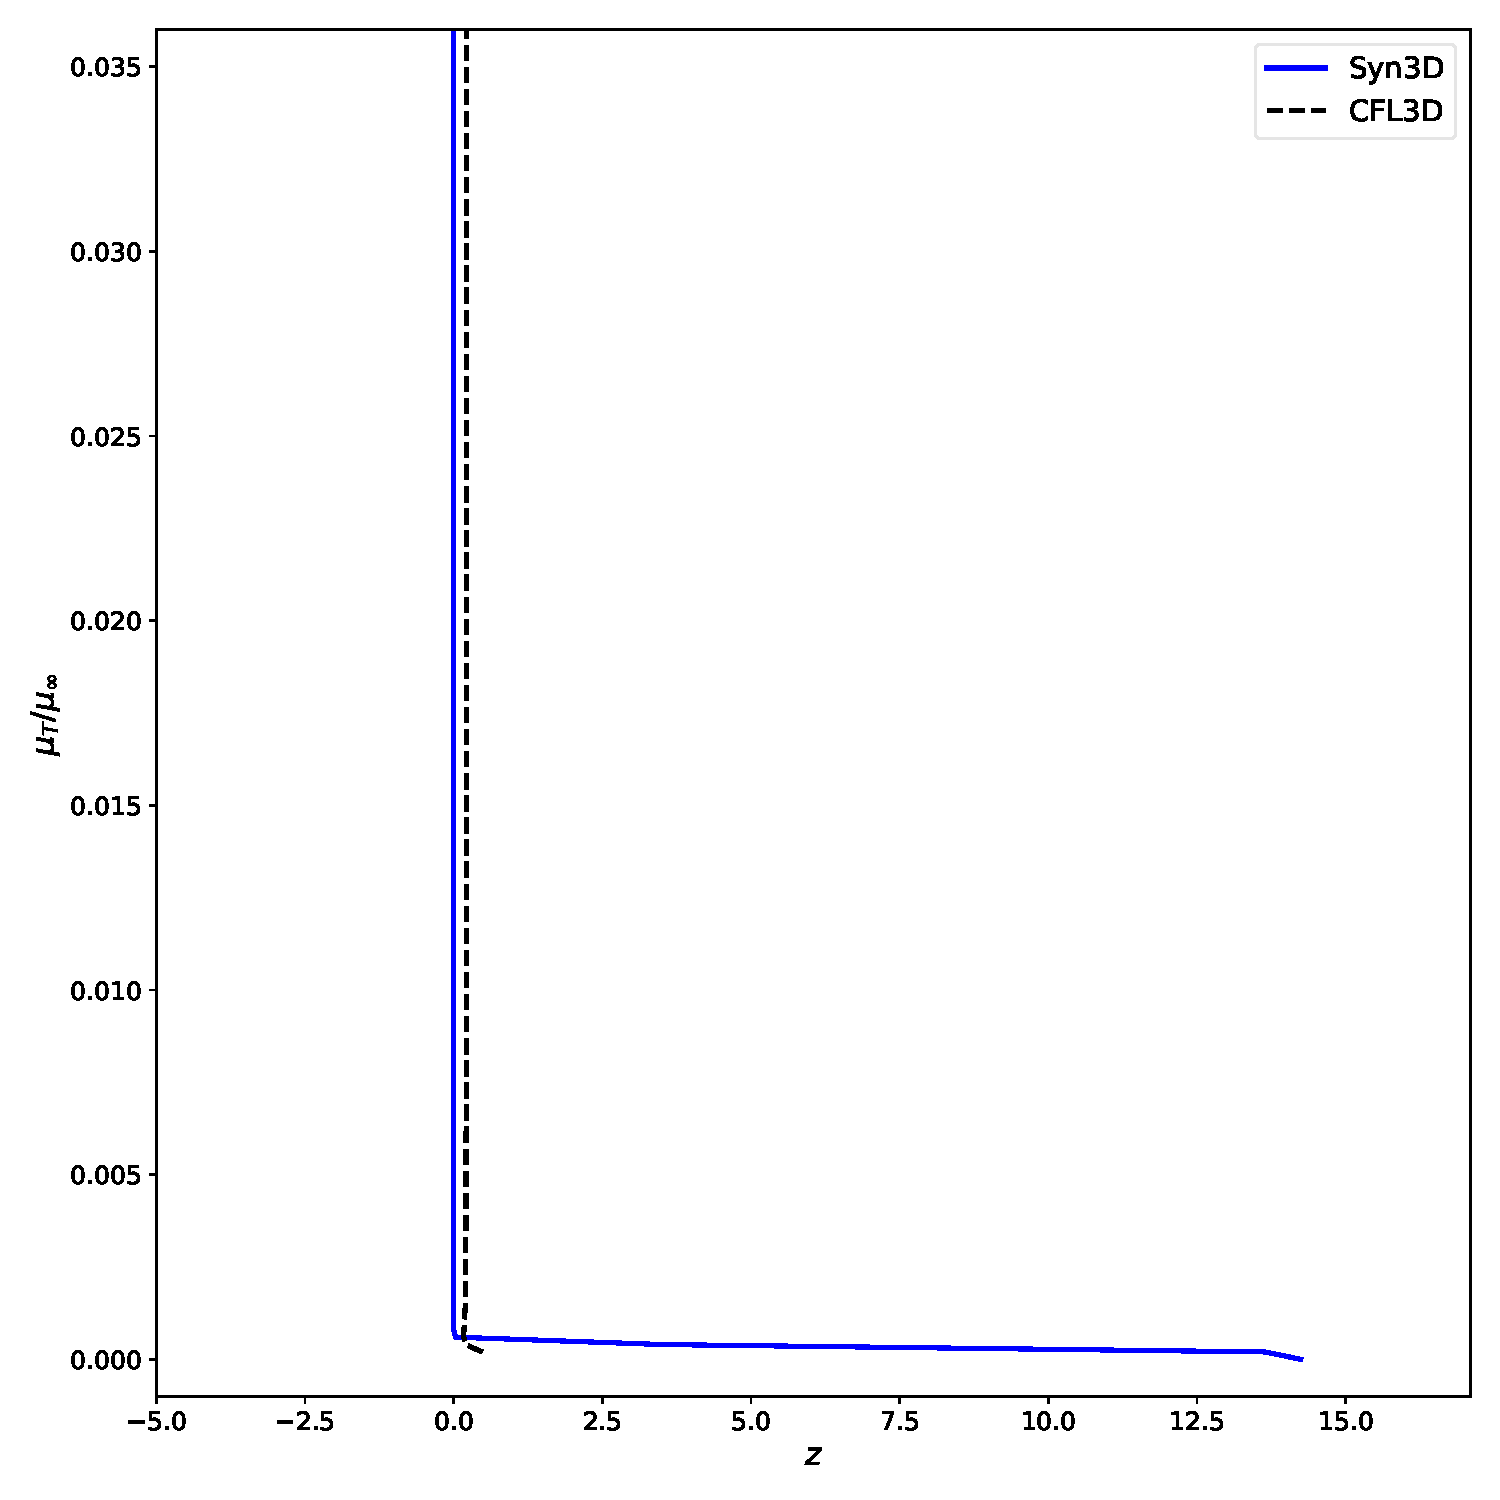
\includegraphics[width=1.0\textwidth]{figs/3dbump/x03y05REV.pdf}
  \caption{$x=0.3, y=-0.5$}
  \label{fig:syn3dbumpbad}
\end{subfigure}%
\\
\begin{subfigure}{.45\textwidth}
  \centering
  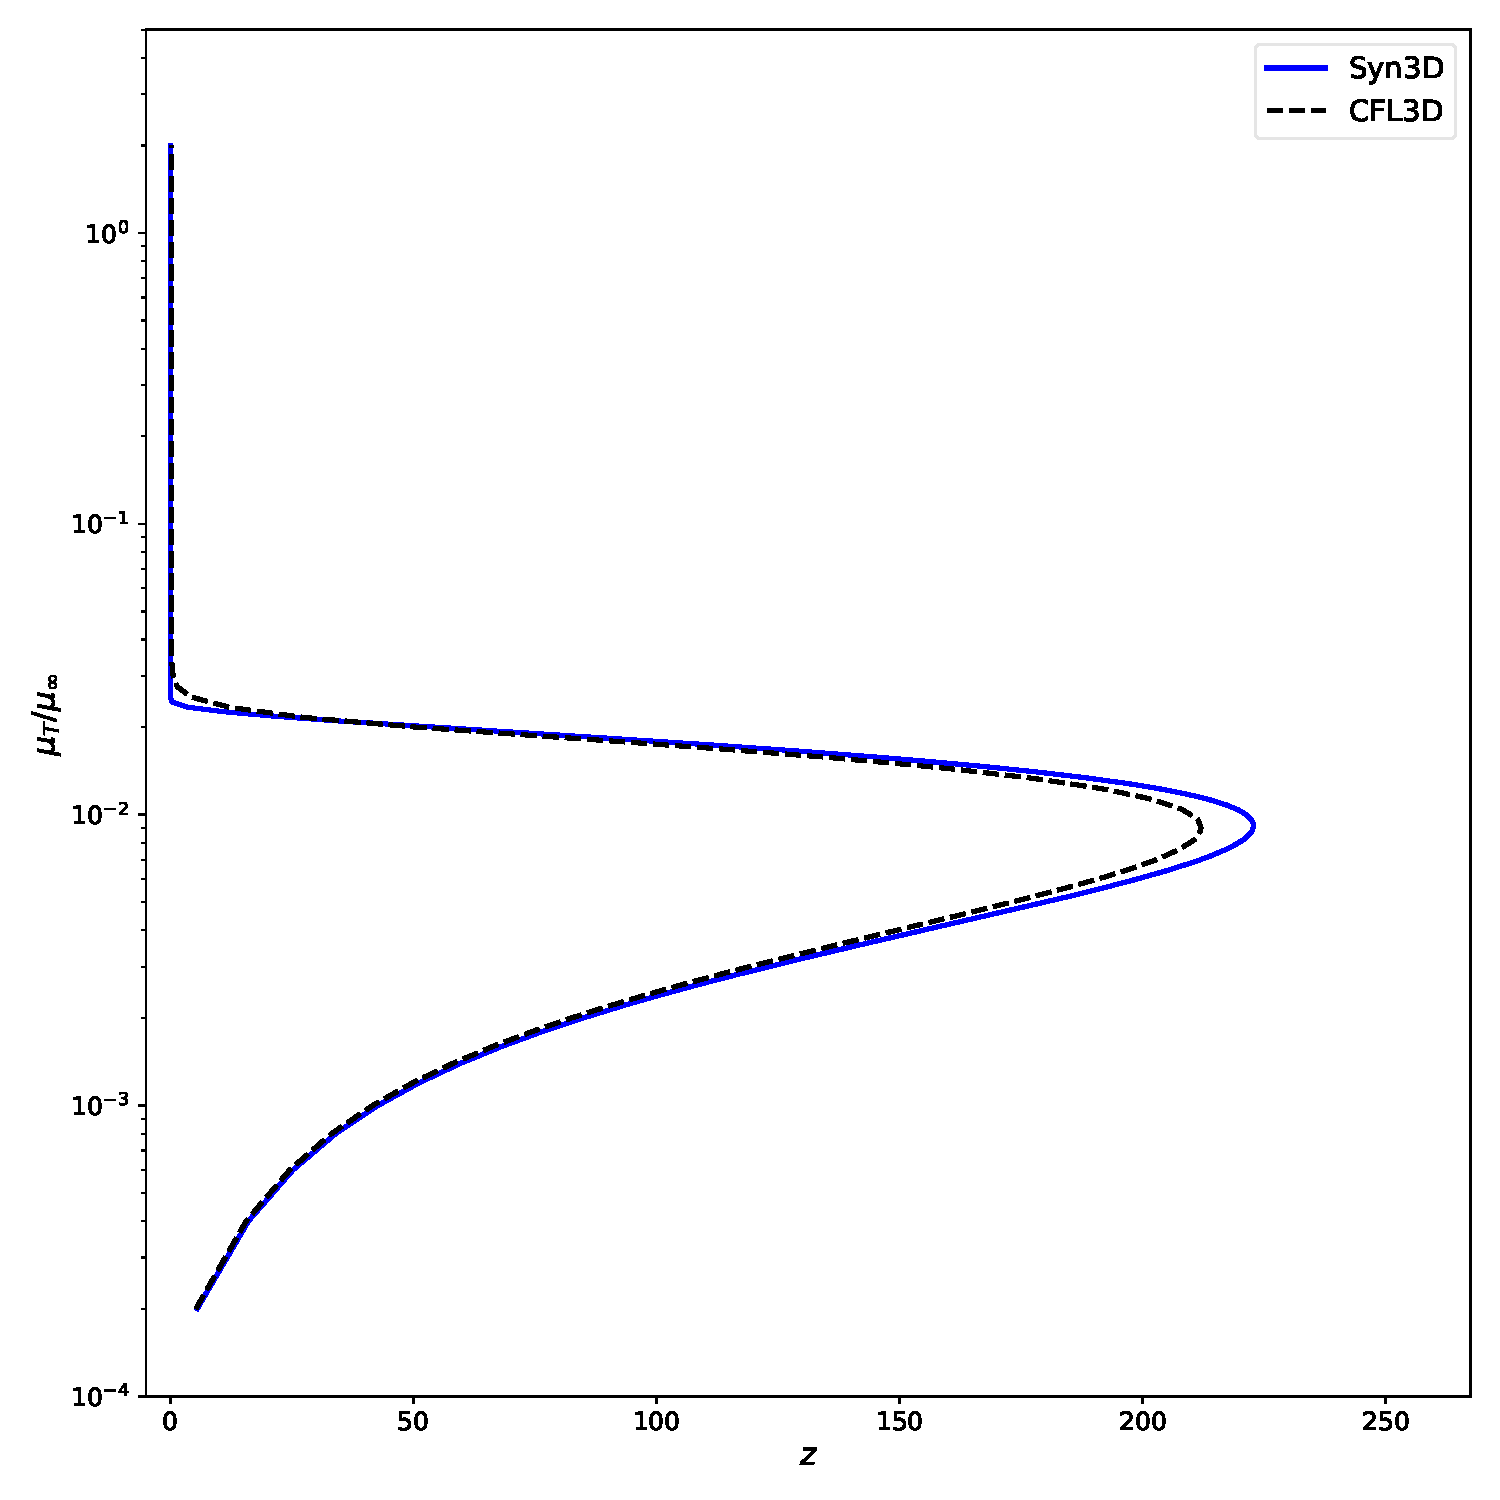
\includegraphics[width=1.0\textwidth]{figs/3dbump/x12y01REV.pdf}
  \caption{$x=1.2, y=-0.1$}
\end{subfigure}%
\begin{subfigure}{.45\textwidth}
  \centering
  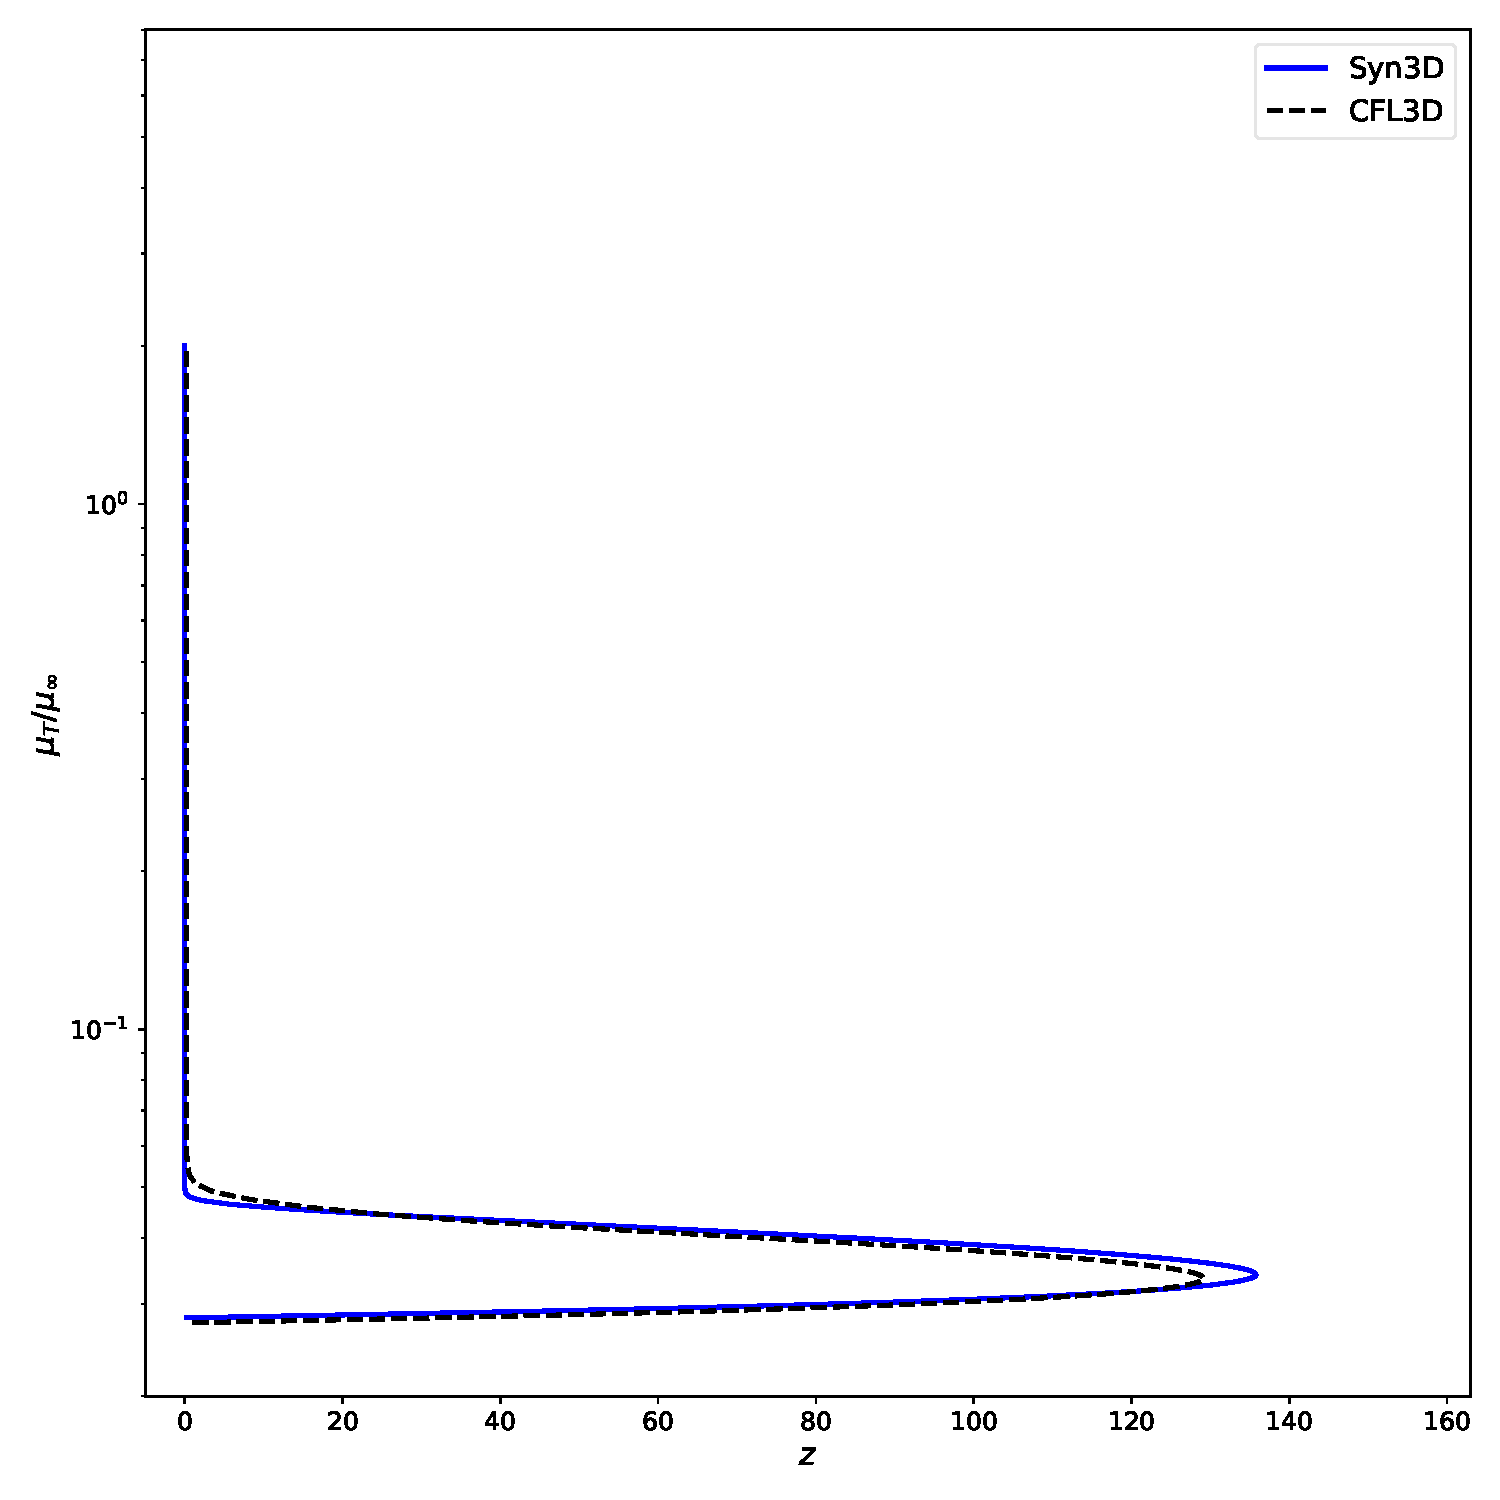
\includegraphics[width=1.0\textwidth]{figs/3dbump/x12y05REV.pdf}
  \caption{$x=1.2, y=-0.5$}
\end{subfigure}%
\caption{3D Bump (syn3D): Comparison of dimensionless eddy viscosity profiles at various locations.}
\label{fig:syn3dbumpmut}
\end{figure}

As for the grid study, \Cref{fig:syn3dbumpforces} compares the dependence of force coefficients on grid size, \Cref{fig:syn3dbumpmutstudy} and \Cref{fig:syn3dbumpcpstudy} compare the eddy viscosity and pressure coefficient at select locations. Similarly to the two-dimensional bump, the pressure contribution to drag is less sensitive to to mesh refinement than the viscous contribution. 
\begin{figure}[ht!]
\centering
\begin{subfigure}{.45\textwidth}
  \centering
  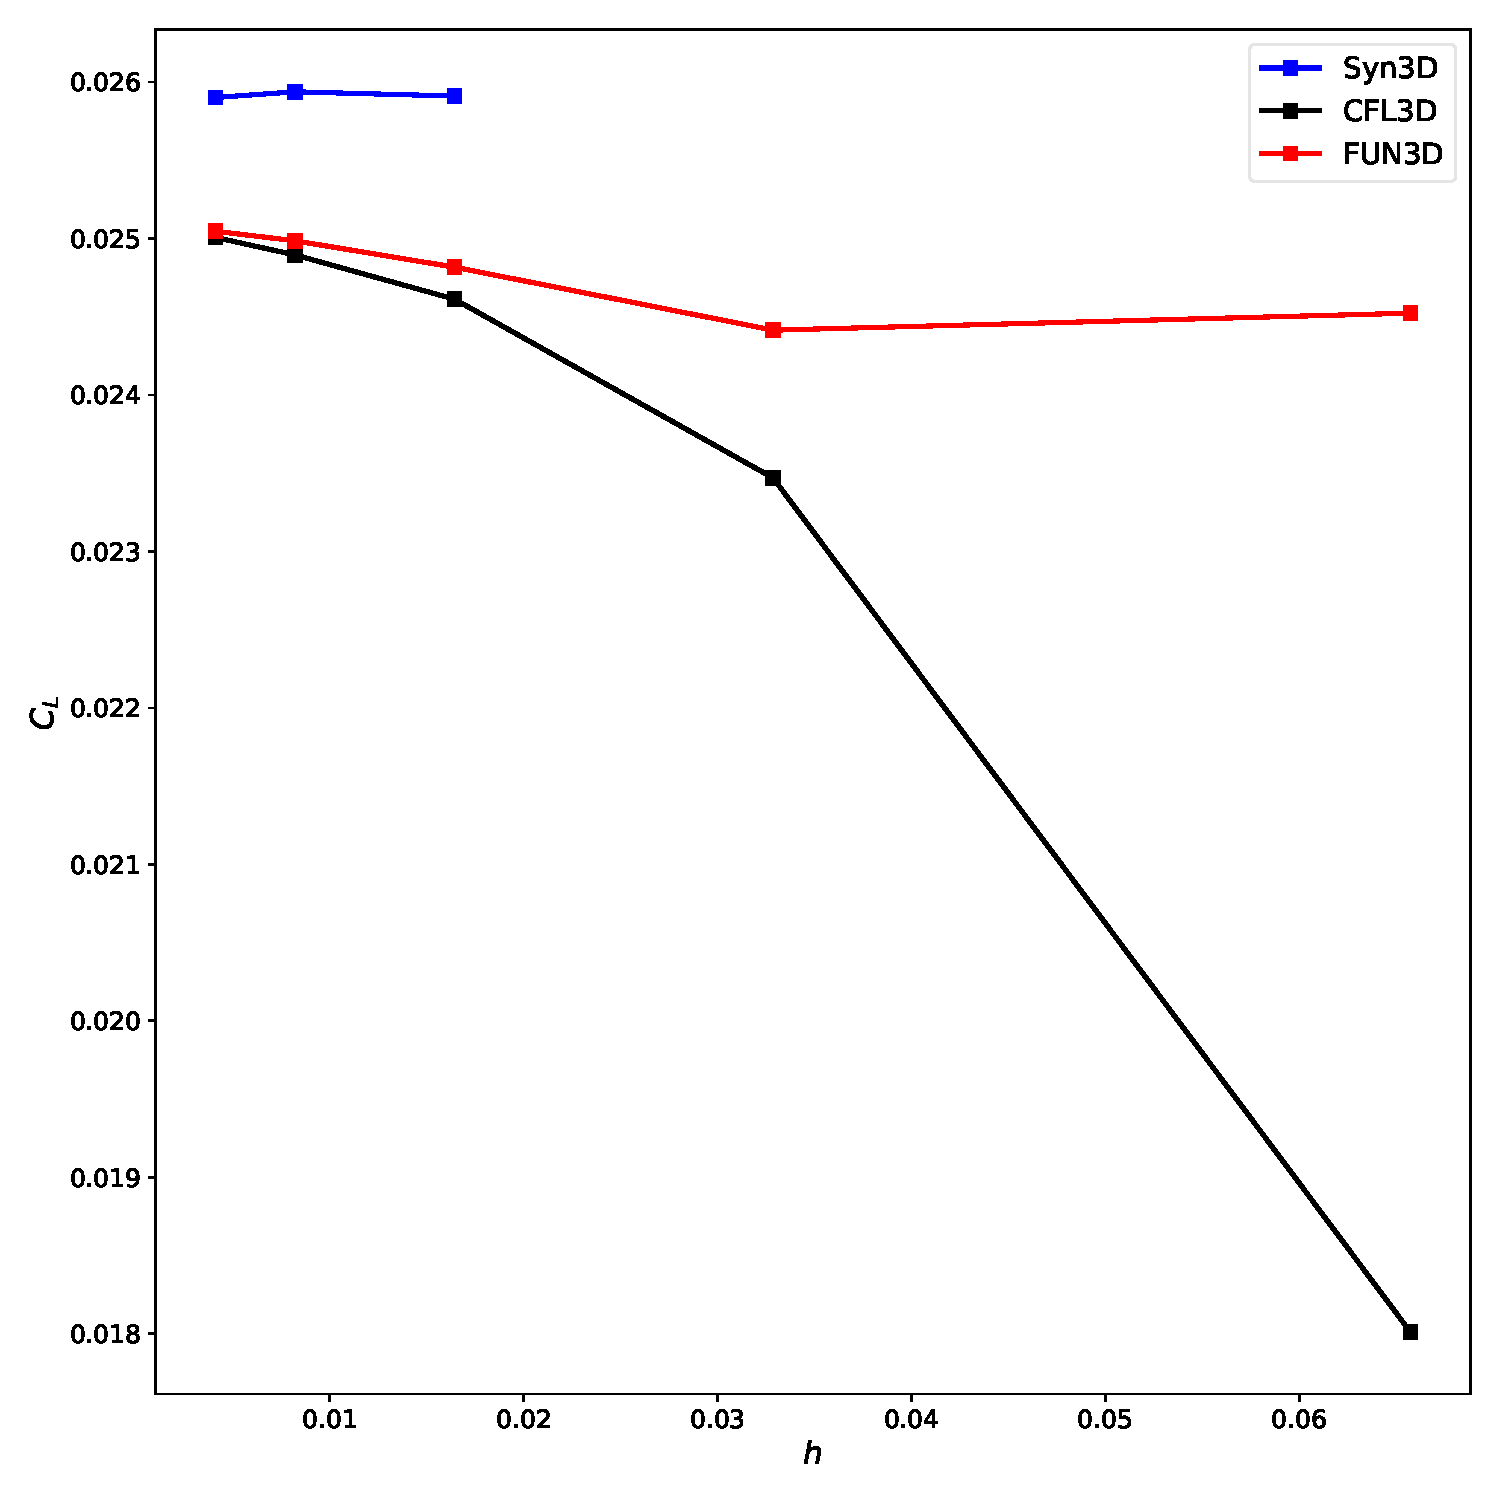
\includegraphics[width=1.0\textwidth]{figs/3dbump/C_L_GridStudy.pdf}
  \caption{$C_L$}
\end{subfigure}%
\begin{subfigure}{.45\textwidth}
  \centering
  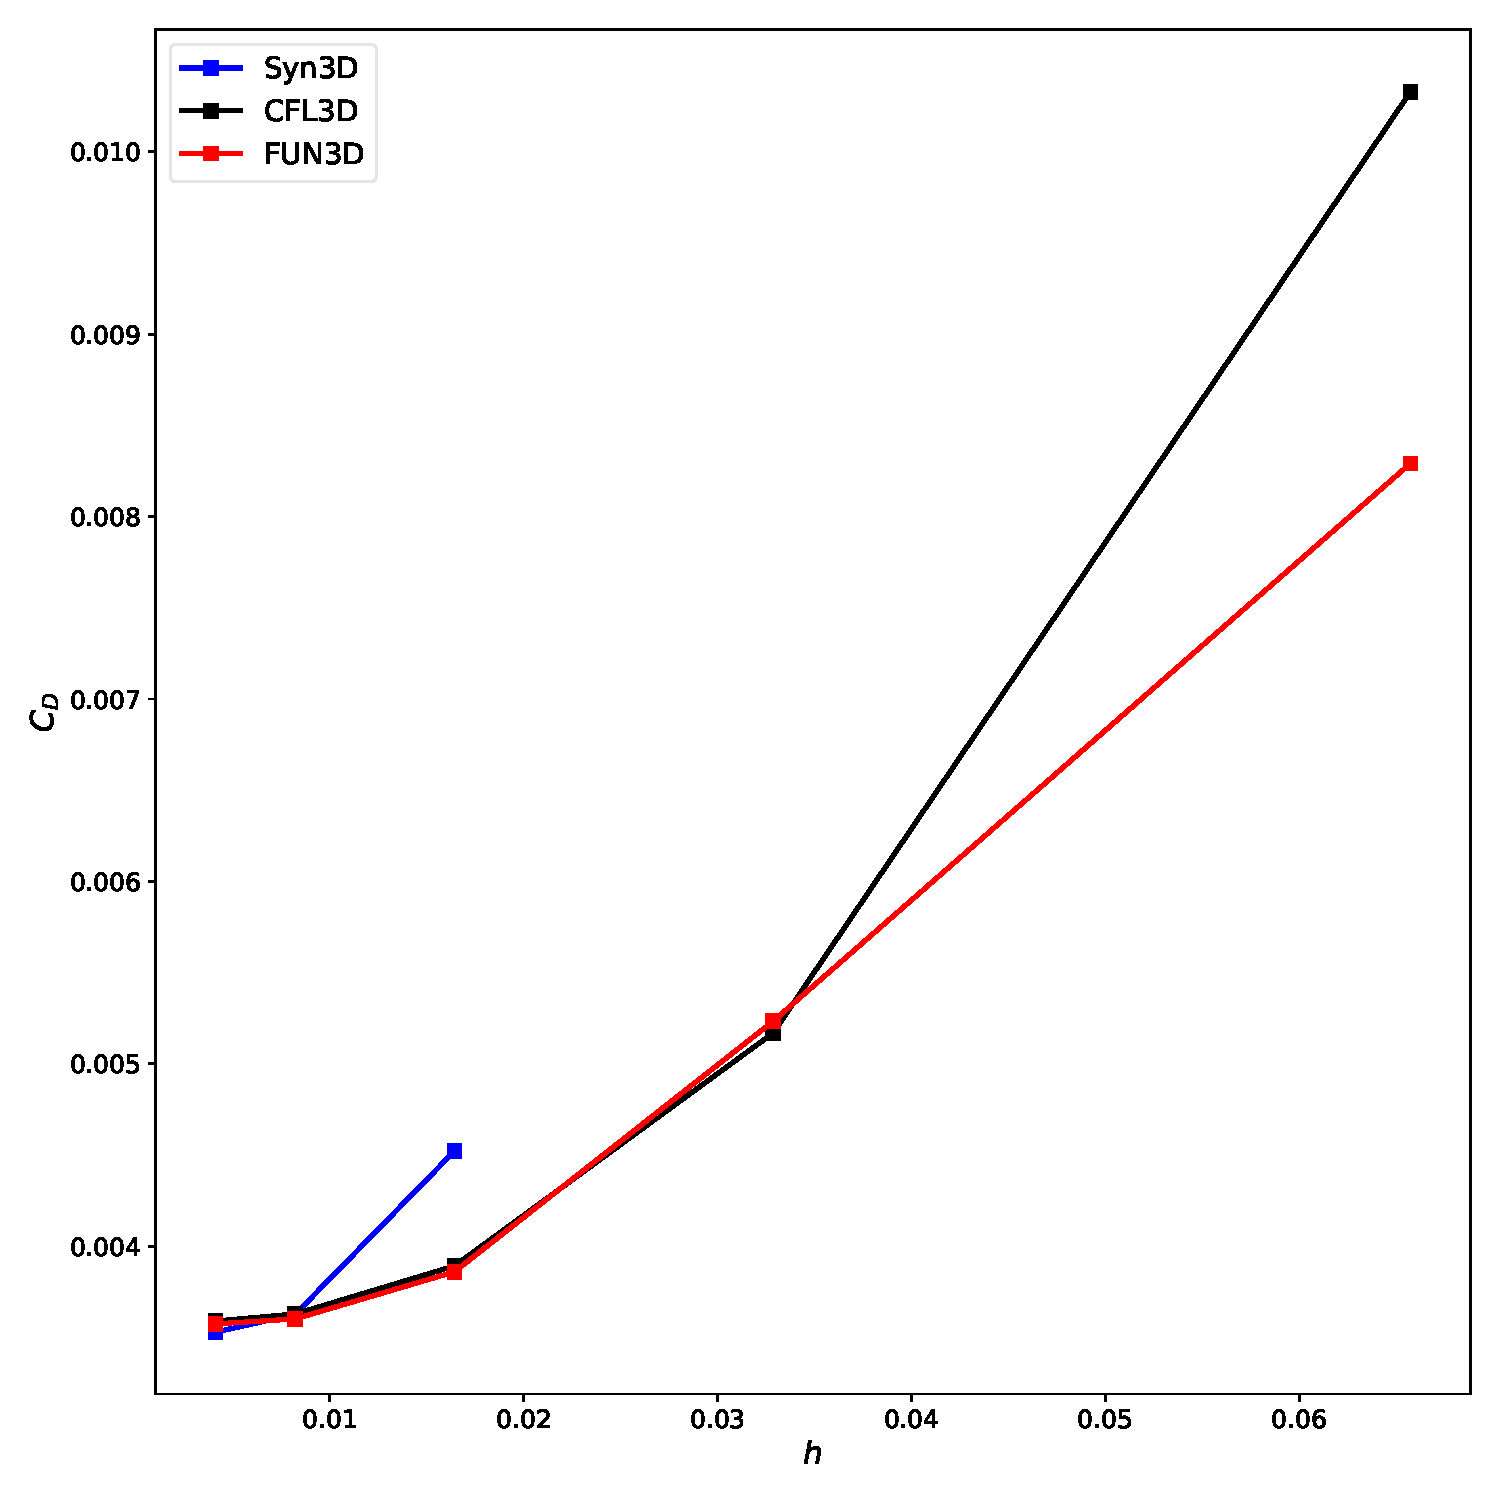
\includegraphics[width=1.0\textwidth]{figs/3dbump/C_D_GridStudy.pdf}
  \caption{$C_D$}
\end{subfigure}
\\
\begin{subfigure}{.45\textwidth}
  \centering
  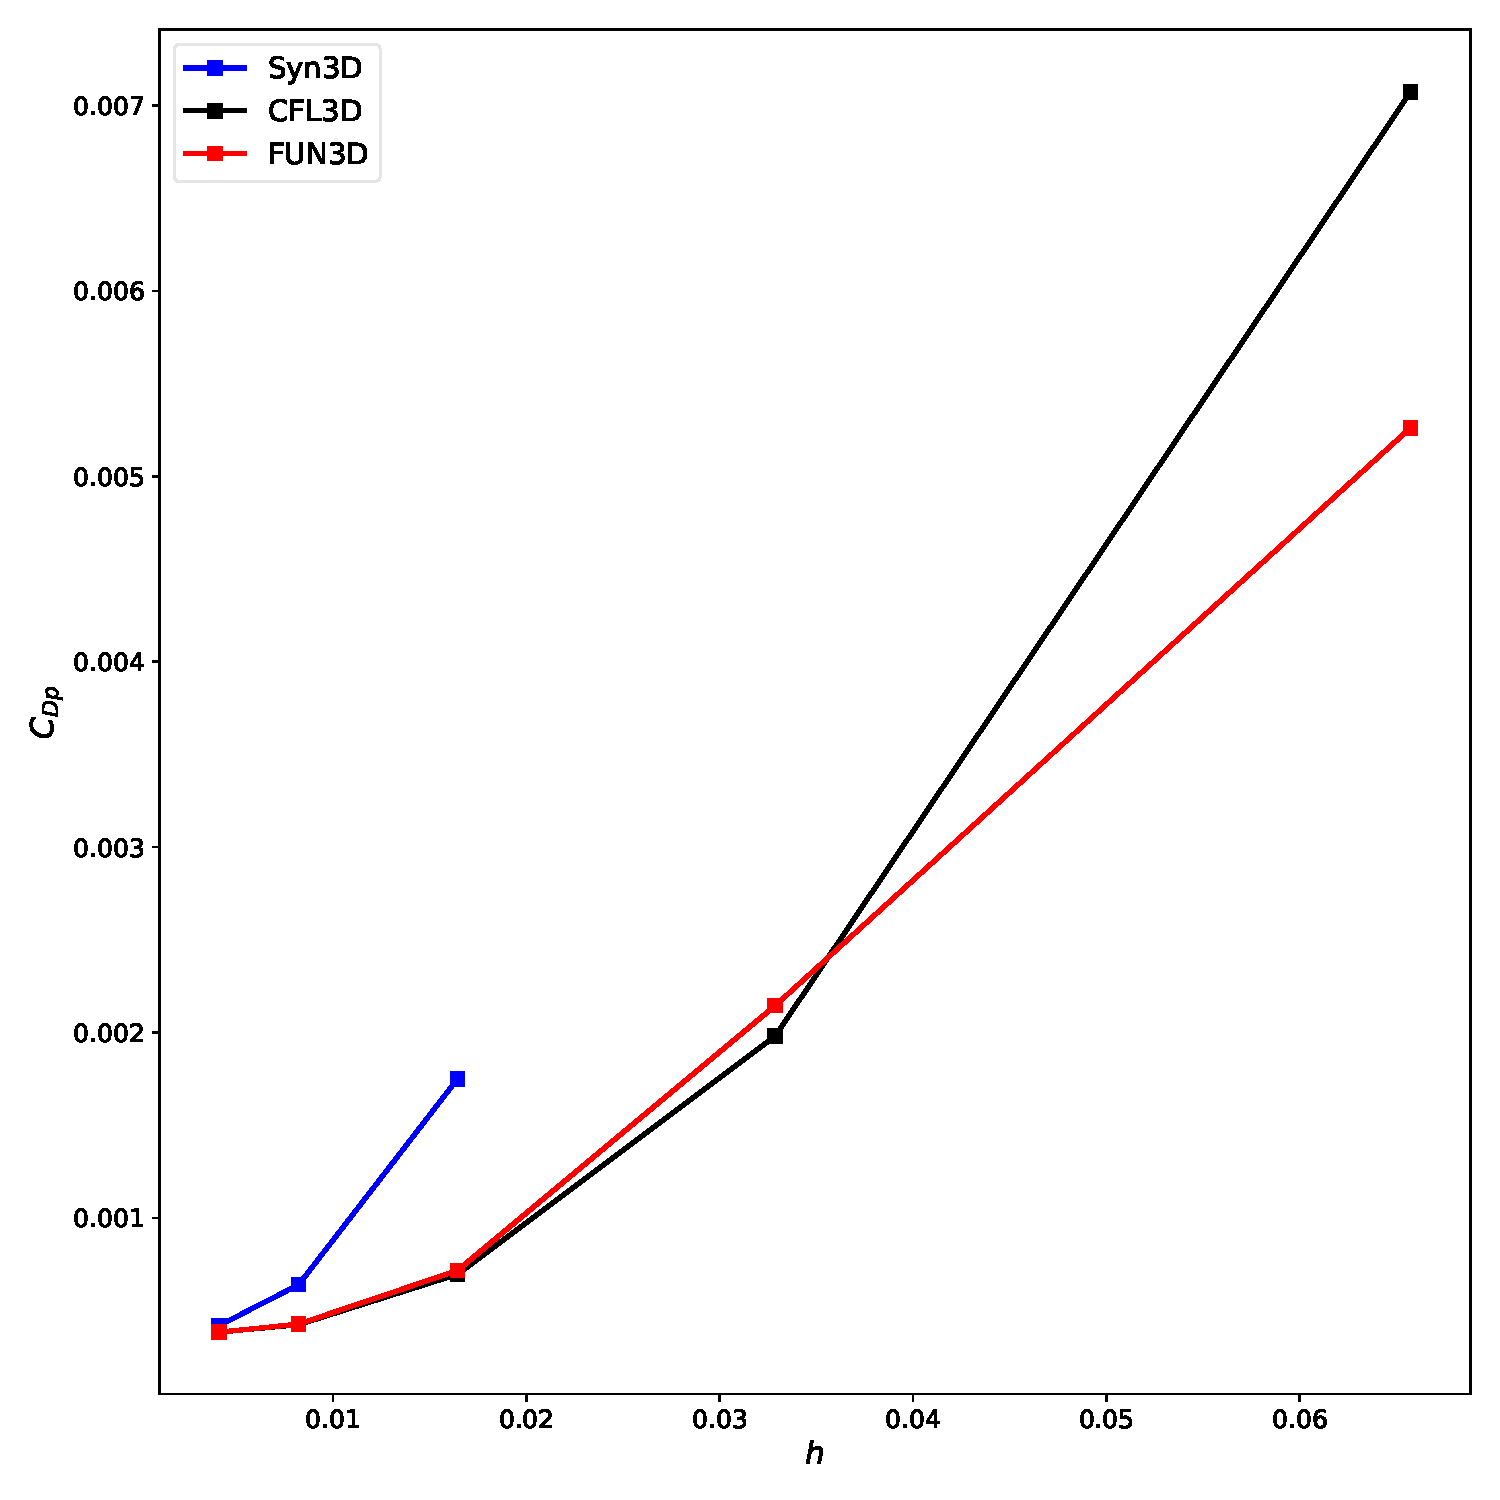
\includegraphics[width=1.0\textwidth]{figs/3dbump/C_Dp_GridStudy.pdf}
  \caption{$C_{Dp}$}
\end{subfigure}%
\begin{subfigure}{.45\textwidth}
  \centering
  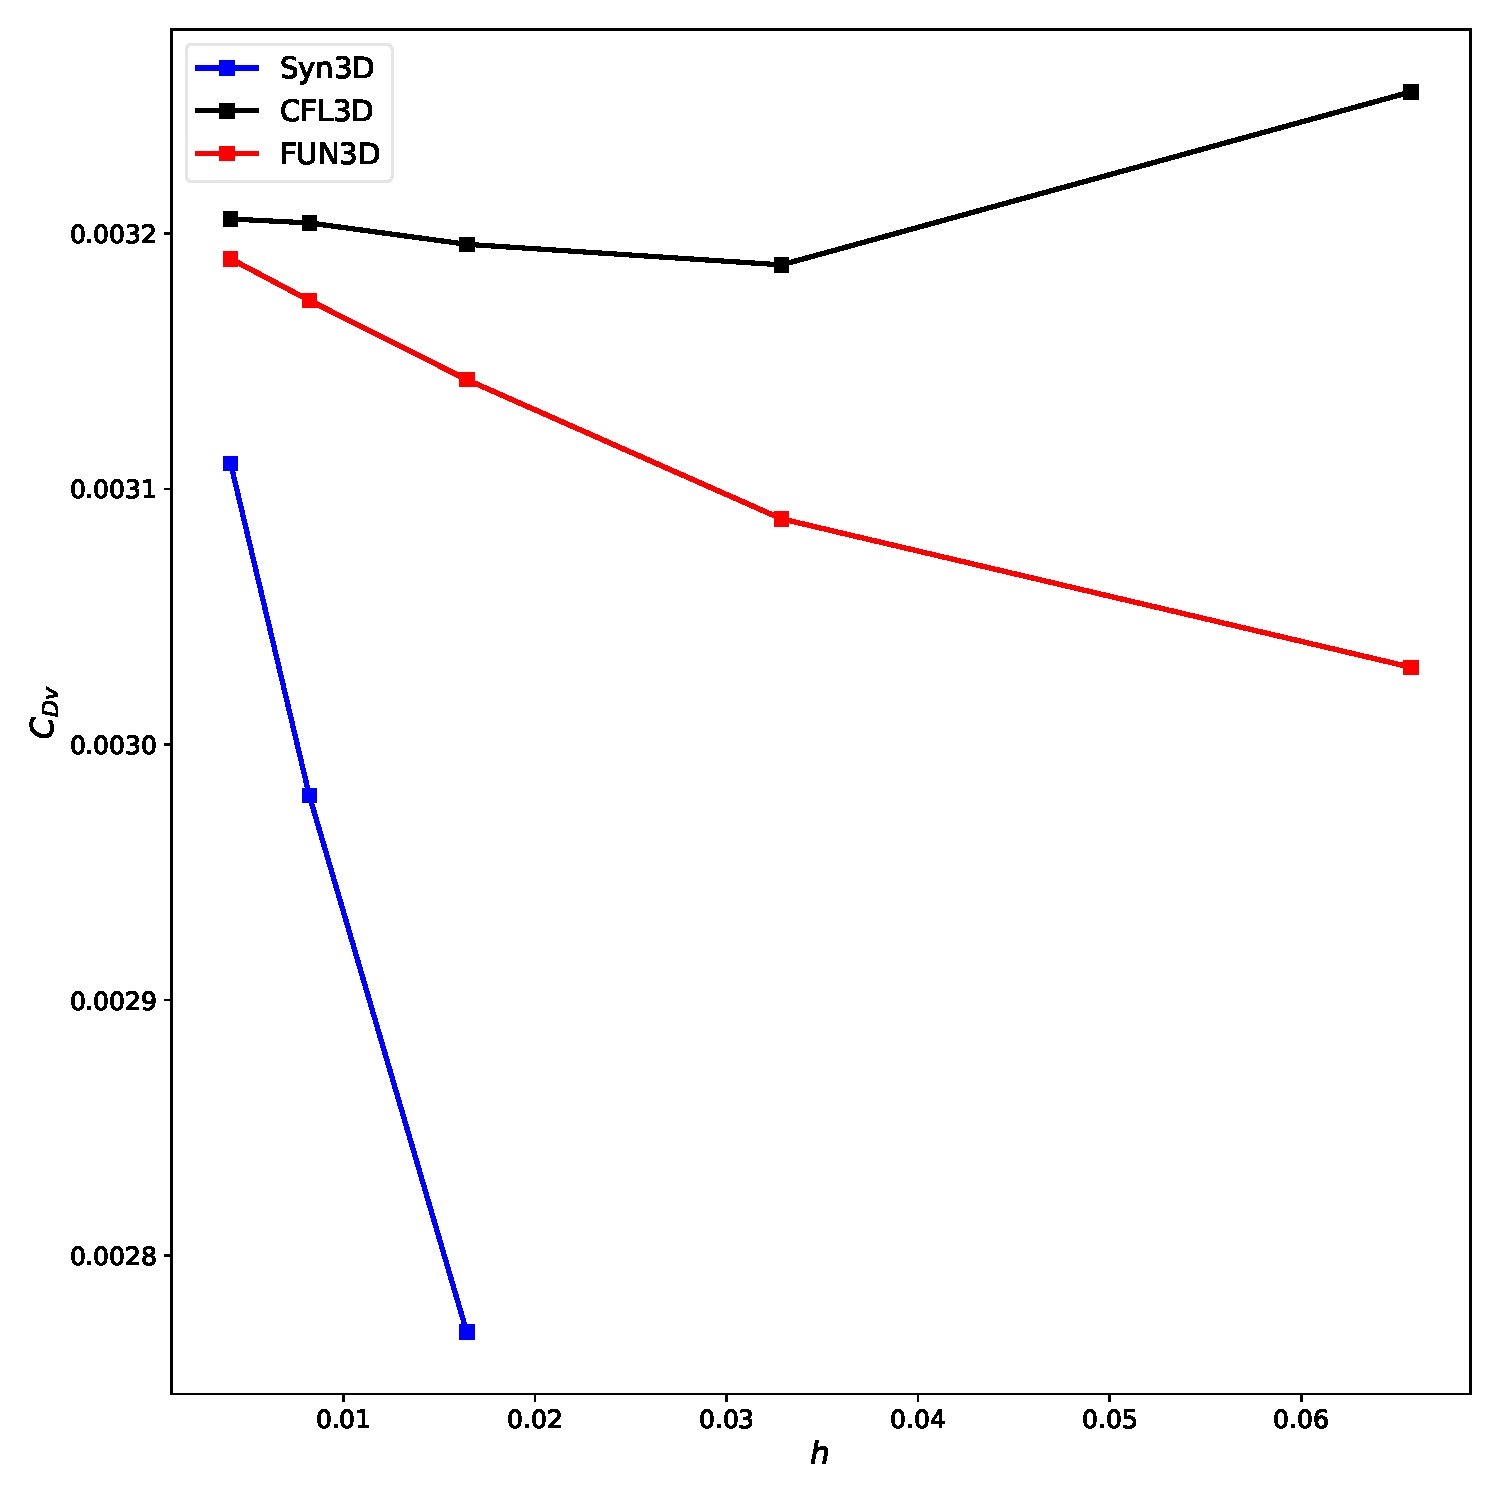
\includegraphics[width=1.0\textwidth]{figs/3dbump/C_Dv_GridStudy.pdf}
  \caption{$C_{Dv}$}
\end{subfigure}
\caption{3D Bump (syn3D): Force coefficients for various grids}
\label{fig:syn3dbumpforces}
\end{figure}

\begin{figure}[ht!]
    \centering
    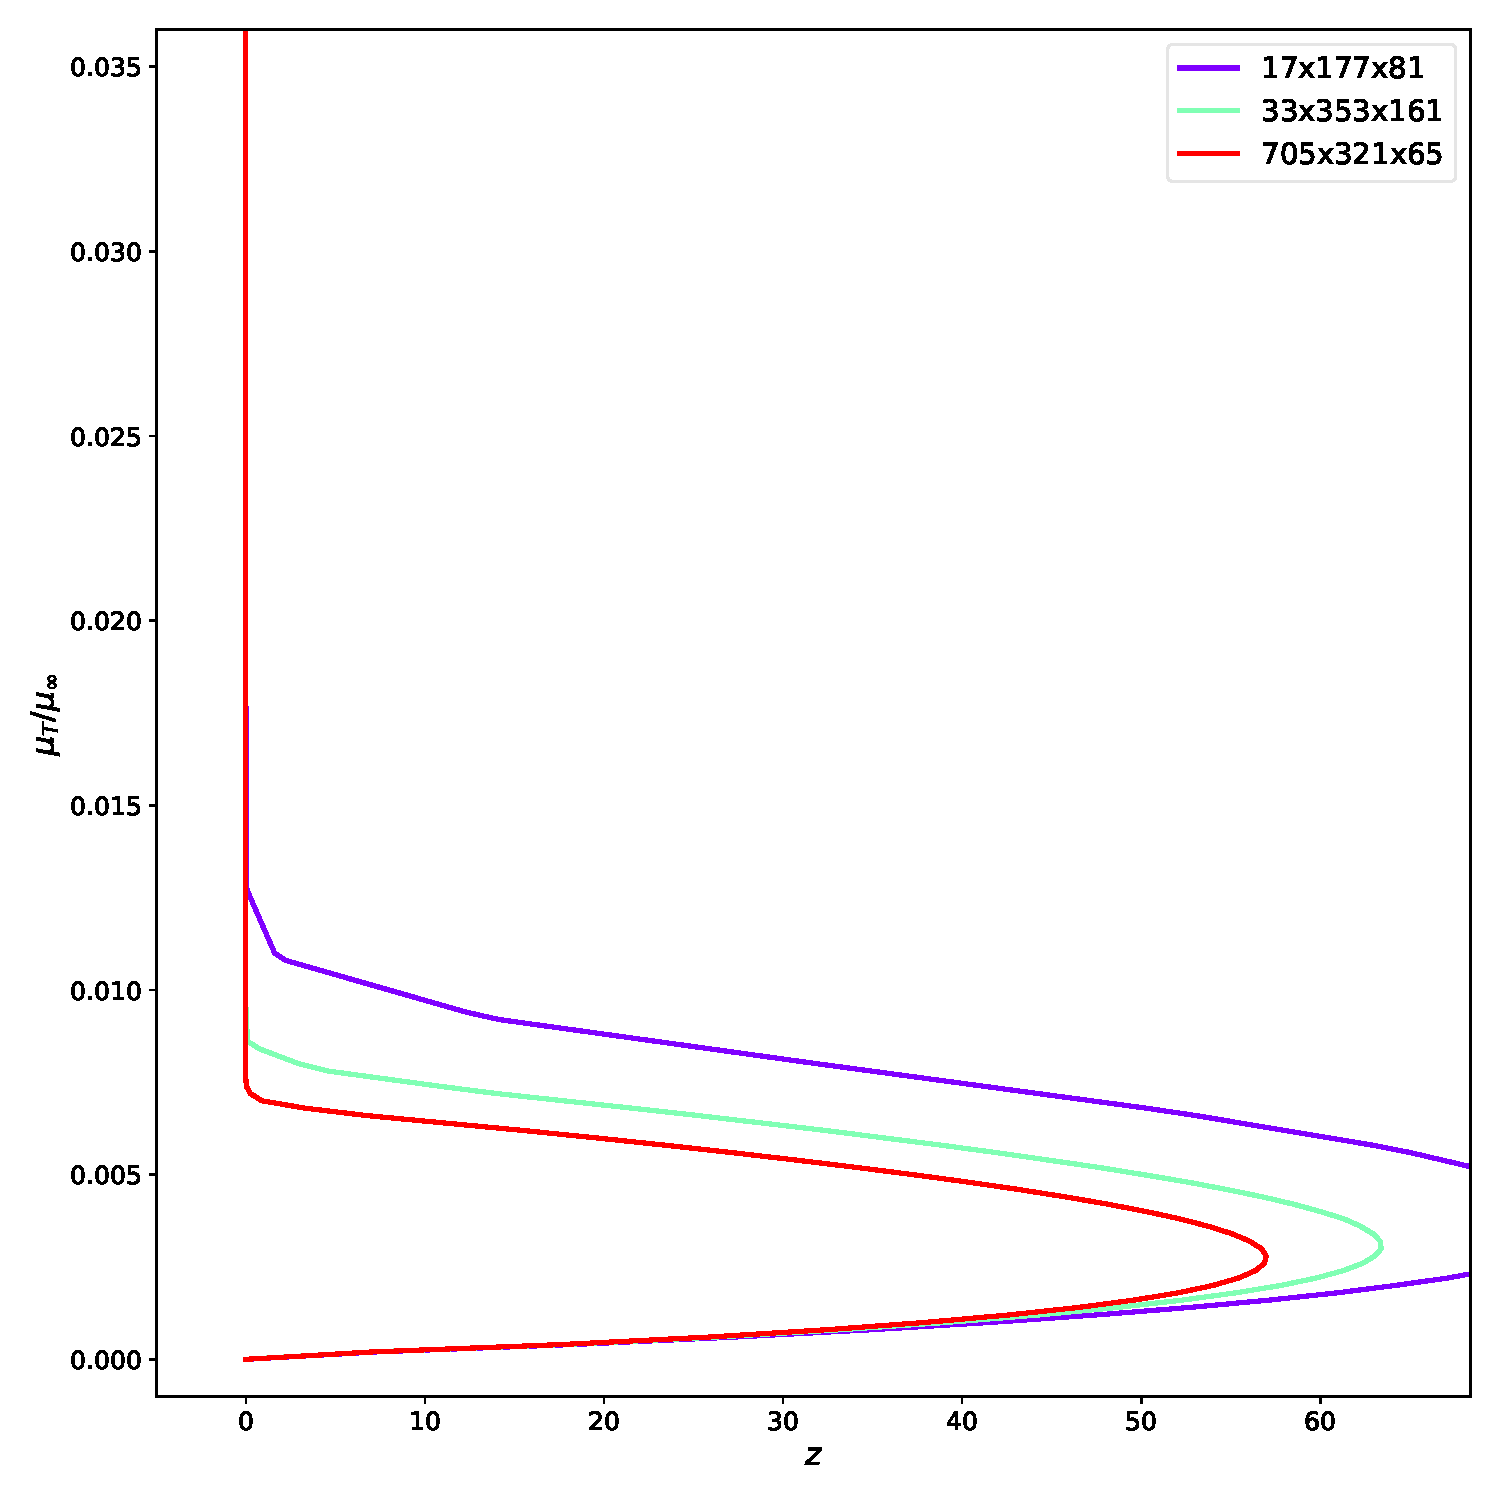
\includegraphics[width=0.4\textwidth]{figs/3dbump/x03y01REV_study.pdf}
    \caption{3D Bump (syn3D): Dimensionless eddy viscosity at $x=0.3,y=0.1$ for various grids.}
    \label{fig:syn3dbumpmutstudy}
\end{figure}

\begin{figure}[ht!]
    \centering
    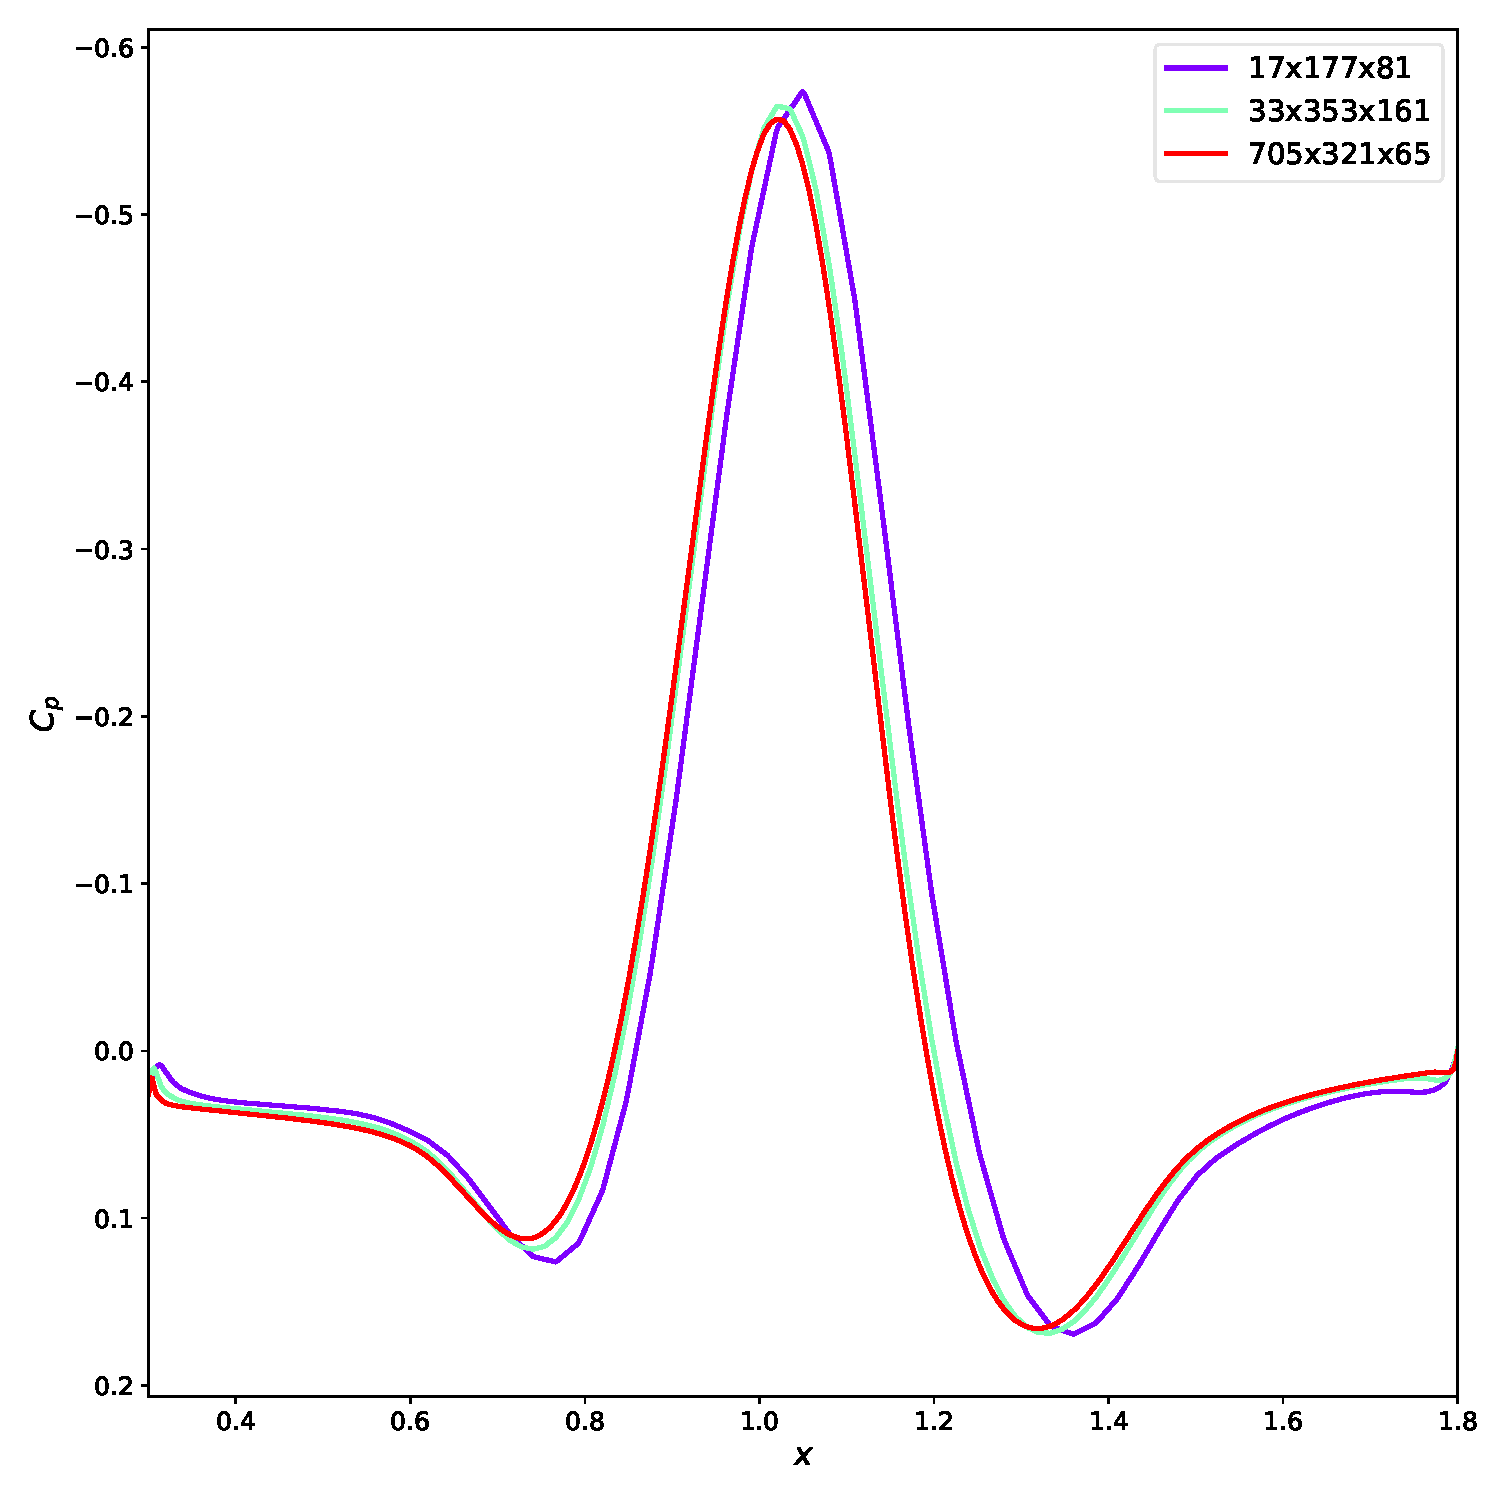
\includegraphics[width=0.4\textwidth]{figs/3dbump/cop050study.pdf}
    \caption{3D Bump (syn3D): Coefficient of pressure at $y=0.5$ for various grids.}
    \label{fig:syn3dbumpcpstudy}
\end{figure}
